\documentclass{beamer}\usepackage[]{graphicx}\usepackage[]{color}
%% maxwidth is the original width if it is less than linewidth
%% otherwise use linewidth (to make sure the graphics do not exceed the margin)
\makeatletter
\def\maxwidth{ %
  \ifdim\Gin@nat@width>\linewidth
    \linewidth
  \else
    \Gin@nat@width
  \fi
}
\makeatother

\definecolor{fgcolor}{rgb}{0.345, 0.345, 0.345}
\newcommand{\hlnum}[1]{\textcolor[rgb]{0.686,0.059,0.569}{#1}}%
\newcommand{\hlstr}[1]{\textcolor[rgb]{0.192,0.494,0.8}{#1}}%
\newcommand{\hlcom}[1]{\textcolor[rgb]{0.678,0.584,0.686}{\textit{#1}}}%
\newcommand{\hlopt}[1]{\textcolor[rgb]{0,0,0}{#1}}%
\newcommand{\hlstd}[1]{\textcolor[rgb]{0.345,0.345,0.345}{#1}}%
\newcommand{\hlkwa}[1]{\textcolor[rgb]{0.161,0.373,0.58}{\textbf{#1}}}%
\newcommand{\hlkwb}[1]{\textcolor[rgb]{0.69,0.353,0.396}{#1}}%
\newcommand{\hlkwc}[1]{\textcolor[rgb]{0.333,0.667,0.333}{#1}}%
\newcommand{\hlkwd}[1]{\textcolor[rgb]{0.737,0.353,0.396}{\textbf{#1}}}%
\let\hlipl\hlkwb

\usepackage{framed}
\makeatletter
\newenvironment{kframe}{%
 \def\at@end@of@kframe{}%
 \ifinner\ifhmode%
  \def\at@end@of@kframe{\end{minipage}}%
  \begin{minipage}{\columnwidth}%
 \fi\fi%
 \def\FrameCommand##1{\hskip\@totalleftmargin \hskip-\fboxsep
 \colorbox{shadecolor}{##1}\hskip-\fboxsep
     % There is no \\@totalrightmargin, so:
     \hskip-\linewidth \hskip-\@totalleftmargin \hskip\columnwidth}%
 \MakeFramed {\advance\hsize-\width
   \@totalleftmargin\z@ \linewidth\hsize
   \@setminipage}}%
 {\par\unskip\endMakeFramed%
 \at@end@of@kframe}
\makeatother

\definecolor{shadecolor}{rgb}{.97, .97, .97}
\definecolor{messagecolor}{rgb}{0, 0, 0}
\definecolor{warningcolor}{rgb}{1, 0, 1}
\definecolor{errorcolor}{rgb}{1, 0, 0}
\newenvironment{knitrout}{}{} % an empty environment to be redefined in TeX

\usepackage{alltt}
\usetheme{default}
%\usetheme{Malmoe}

\title[EC999: Quantitative Text Analysis]{EC999: Sourcing Data} \def\newblock{\hskip .11em plus .33em minus .07em}


\def\Tiny{\fontsize{10pt}{10pt}\selectfont}
\def\smaller{\fontsize{8pt}{8pt}\selectfont}

\institute[Warwick]{University of Chicago \& University of Warwick}
\author[Thiemo Fetzer]{Thiemo Fetzer}

 \date{\today}

\usepackage{natbib}
\usepackage{amsmath}
\usepackage{hyperref}
\usepackage{graphicx}
\usepackage{graphics}

\usepackage{amsfonts}
\usepackage{amssymb}
\usepackage{pdfpages}
\usepackage{natbib}
\usepackage{hyperref}
%\usepackage{enumitem}
 \usepackage{pgffor}
\usepackage{booktabs,caption,fixltx2e}
\usepackage[flushleft]{threeparttable}
\usepackage{verbatim} 
\usepackage{cancel}
\newcommand\xxcancel[1]{\xcancel{#1}\vphantom{#1}}

\usepackage{mathtools,xparse}

\newenvironment{Description}
               {\list{}{\labelwidth=0pt \itemindent-\leftmargin
                        \let\makelabel\Descriptionlabel
                        % or whatever
               }}
               {\endlist}
\newcommand*\Descriptionlabel[1]{%
  \hspace\labelsep
  \normalfont%  reset current font setting
  \color{blue}\bfseries\sffamily% or whatever 
  #1}


\setbeamersize{text margin left = 16pt, text margin right = 16pt}
\newcommand{\code}[1]{\texttt{#1}}

\newenvironment<>{algorithm}[1][\undefined]{%
\begin{actionenv}#2%
\ifx#1\undefined%
   \def\insertblocktitle{Algorithm}%
\else%
   \def\insertblocktitle{Algorithm ({\em#1})}%
\fi%
\par%
\mode<presentation>{%
  \setbeamercolor{block title}{fg=white,bg=yellow!50!black}
  \setbeamercolor{block body}{fg=black,bg=yellow!20}
}%
\usebeamertemplate{block begin}\em}
{\par\usebeamertemplate{block end}\end{actionenv}}


\newenvironment<>{assumption}[1][\undefined]{%
\begin{actionenv}#2%
\ifx#1\undefined%
   \def\insertblocktitle{Assumption}%
\else%
   \def\insertblocktitle{Assumption ({\em#1})}%
\fi%
\par%
\mode<presentation>{%
  \setbeamercolor{block title}{fg=white,bg=blue!50!black}
  \setbeamercolor{block body}{fg=black,bg=blue!20}
}%
\usebeamertemplate{block begin}\em}
{\par\usebeamertemplate{block end}\end{actionenv}}


\usepackage{etoolbox} 
\makeatletter 
\preto{\@verbatim}{\topsep=0pt \partopsep=0pt } 
\makeatother
\renewenvironment{knitrout}{\setlength{\topsep}{0mm}}{}
\IfFileExists{upquote.sty}{\usepackage{upquote}}{}
\begin{document}



\AtBeginSection[]
{
 \begin{frame}<beamer>
 \frametitle{Plan}
 \tableofcontents[currentsection]
 \end{frame}
}
\maketitle
 

%%%%%%%%%%%%%%%%%%%%%%%%%%%%



\section{Basic String Manipulation}
%%%%%%%%%%%%%%%%%%%%%%%%%%%%%%%%%%%%%%%%%%%%%%%%%%%%%%%%%%
\begin{frame}[fragile]{Basic Manipulating of Strings in R}
After introducing the R-basics in the last lecture, we will turn to the basics of string manipulation. 
\begin{itemize}

\item Basic string manipulation functions

\item Regular Expressions, search and replace

\end{itemize}

Top string manipulation functions: - \code{tolower} (also \code{toupper}, capitalize) - \code{nchar} - \code{grep} - \code{gsub} - \code{substring} - \code{paste} and \code{paste0} - and the following from library stringr: \code{strtrim} , \code{str\_extract}, \code{str\_match}, \code{str\_split} but many more.
\end{frame}
%%%%%%%%%%%%%%%%%%%%%%%%%%%%%%%%%%%%%%%%%%%%%%%%%%%%%%%%%%%%%%%%%%%%%%%%%

%%%%%%%%%%%%%%%%%%%%%%%%%%%%%%%%%%%%%%%%%%%%%%%%%%%%%%%%%%
\begin{frame}[fragile]{Case-folding for dimensionality reduction} 

As we will see, due to the curse of dimensionality, we will often simply ignore the case o individual words, as depending on the task at hand, the word case does not carry a lot of information.

\begin{knitrout}\tiny
\definecolor{shadecolor}{rgb}{0.969, 0.969, 0.969}\color{fgcolor}\begin{kframe}
\begin{alltt}
\hlcom{#USArrests is a data frame that R comes shipped with }
\hlstd{states} \hlkwb{=} \hlkwd{rownames}\hlstd{(USArrests)}
\hlkwd{tolower}\hlstd{(states[}\hlnum{0}\hlopt{:}\hlnum{4}\hlstd{])}
\end{alltt}
\begin{verbatim}
## [1] "alabama"  "alaska"   "arizona"  "arkansas"
\end{verbatim}
\begin{alltt}
\hlkwd{toupper}\hlstd{(states[}\hlnum{0}\hlopt{:}\hlnum{4}\hlstd{])}
\end{alltt}
\begin{verbatim}
## [1] "ALABAMA"  "ALASKA"   "ARIZONA"  "ARKANSAS"
\end{verbatim}
\begin{alltt}
\hlcom{#smarter way to do case folding is not to replace acronyms like US or IBM, }
\hlcom{#for that use regular expressions (see later)}
\hlstd{WORDS}\hlkwb{<-}\hlkwd{c}\hlstd{(}\hlstr{"IBM"}\hlstd{,} \hlstr{"Chicago"}\hlstd{)}

\hlstd{WORDS[}\hlkwd{grep}\hlstd{(}\hlstr{"[^A-Z]\{2,\}[a-z]*"}\hlstd{,WORDS)]}\hlkwb{<-}\hlkwd{tolower}\hlstd{(WORDS[}\hlkwd{grep}\hlstd{(}\hlstr{"[^A-Z]\{2,\}[a-z]*"}\hlstd{,WORDS)])}

\hlstd{WORDS}
\end{alltt}
\begin{verbatim}
## [1] "IBM"     "chicago"
\end{verbatim}
\end{kframe}
\end{knitrout}

\end{frame}
%%%%%%%%%%%%%%%%%%%%%%%%%%%%%%%%%%%%%%%%%%%%%%%%%%%%%%%%%%%%%%%%%%%%%%%%%


%%%%%%%%%%%%%%%%%%%%%%%%%%%%%%%%%%%%%%%%%%%%%%%%%%%%%%%%%%
\begin{frame}[fragile]{Number of Characters and Substr} 

Note - whitespaces count as characters.

\begin{knitrout}\tiny
\definecolor{shadecolor}{rgb}{0.969, 0.969, 0.969}\color{fgcolor}\begin{kframe}
\begin{alltt}
\hlkwd{nchar}\hlstd{(states)}
\end{alltt}
\begin{verbatim}
##  [1]  7  6  7  8 10  8 11  8  7  7  6  5  8  7  4  6  8  9  5  8 13  8  9 11  8  7  8  6
## [29] 13 10 10  8 14 12  4  8  6 12 12 14 12  9  5  4  7  8 10 13  9  7
\end{verbatim}
\begin{alltt}
\hlstd{states[}\hlkwd{which}\hlstd{(}\hlkwd{nchar}\hlstd{(states)}\hlopt{==}\hlnum{5}\hlstd{)]}
\end{alltt}
\begin{verbatim}
## [1] "Idaho" "Maine" "Texas"
\end{verbatim}
\begin{alltt}
\hlkwd{library}\hlstd{(stringr)}

\hlcom{#trim leading and trailing white spaces at beginning and end of string}
\hlkwd{str_trim}\hlstd{(}\hlstr{" This is a test  .  "}\hlstd{)}
\end{alltt}
\begin{verbatim}
## [1] "This is a test  ."
\end{verbatim}
\begin{alltt}
\hlcom{#get a substring substr(x, start, stop)}
\hlkwd{substr}\hlstd{(states[}\hlnum{1}\hlstd{],} \hlnum{3}\hlstd{,} \hlkwd{nchar}\hlstd{(states[}\hlnum{1}\hlstd{]))}
\end{alltt}
\begin{verbatim}
## [1] "abama"
\end{verbatim}
\end{kframe}
\end{knitrout}

\end{frame}
%%%%%%%%%%%%%%%%%%%%%%%%%%%%%%%%%%%%%%%%%%%%%%%%%%%%%%%%%%%%%%%%%%%%%%%%%


%%%%%%%%%%%%%%%%%%%%%%%%%%%%%%%%%%%%%%%%%%%%%%%%%%%%%%%%%%
\begin{frame}[fragile]{Splitting Strings} 

A simple word or sentence tokenizer works off splitting near white spaces or sentences.
\begin{knitrout}\tiny
\definecolor{shadecolor}{rgb}{0.969, 0.969, 0.969}\color{fgcolor}\begin{kframe}
\begin{alltt}
\hlstd{link}\hlkwb{=}\hlstr{"http://stats.grok.se/json/en/201401/Donald_Trump"}
\hlkwd{str_split}\hlstd{(link,}\hlstr{'/'}\hlstd{)}
\end{alltt}
\begin{verbatim}
## [[1]]
## [1] "http:"         ""              "stats.grok.se" "json"          "en"           
## [6] "201401"        "Donald_Trump"
\end{verbatim}
\begin{alltt}
\hlstd{sentence}\hlkwb{=}\hlstr{"This is a sentence that is split by white spaces."}
\hlkwd{str_split}\hlstd{(sentence,}\hlstr{' '}\hlstd{)}
\end{alltt}
\begin{verbatim}
## [[1]]
##  [1] "This"     "is"       "a"        "sentence" "that"     "is"       "split"   
##  [8] "by"       "white"    "spaces."
\end{verbatim}
\begin{alltt}
\hlcom{#str_split accepts regexes as split patterns}
\hlstd{sentence}\hlkwb{=}\hlstr{"Two sentences example. The split occurs around full-stops followed by white space."}
\hlkwd{str_split}\hlstd{(sentence,}\hlstr{'\textbackslash{}\textbackslash{}. '}\hlstd{)}
\end{alltt}
\begin{verbatim}
## [[1]]
## [1] "Two sentences example"                                      
## [2] "The split occurs around full-stops followed by white space."
\end{verbatim}
\end{kframe}
\end{knitrout}

\end{frame}
%%%%%%%%%%%%%%%%%%%%%%%%%%%%%%%%%%%%%%%%%%%%%%%%%%%%%%%%%%%%%%%%%%%%%%%%%



%%%%%%%%%%%%%%%%%%%%%%%%%%%%%%%%%%%%%%%%%%%%%%%%%%%%%%%%%%
\begin{frame}[fragile]{Regular Expressions} 

\begin{itemize}

\item The first Information Retrieval pipelines working off textual data were making heavy use of regular expressions.

\item Regular expressions, as the name indicates, is a pattern that describes a set of strings.

\item If a string matches a regular expression, it indicates that the presented string follows the pattern of the regular expression.
\end{itemize}

\end{frame}
%%%%%%%%%%%%%%%%%%%%%%%%%%%%%%%%%%%%%%%%%%%%%%%%%%%%%%%%%%%%%%%%%%%%%%%%%


%%%%%%%%%%%%%%%%%%%%%%%%%%%%%%%%%%%%%%%%%%%%%%%%%%%%%%%%%%
\begin{frame}[fragile]{Regex Character Classes} 

\begin{itemize}

\item \code{[a-z]} : lower case letters

\item \code{[0-9]} or \code{[[:digit:]]}: Digits: 0 1 2 3 4 5 6 7 8 9.

\item \code{[[:alnum:]]}
Alphanumeric characters: \code{[[:alpha:]]} and \code{[[:digit:]]}.

\item \code{[[:alpha:]]}
Alphabetic characters: \code{[[:lower:]]} and \code{[[:upper:]]}.

\item \code{[[:blank:]]}
Blank characters: space and tab, and possibly other locale-dependent characters such as non-breaking space.


\item \code{[[:lower:]]} or  \code{[[:upper:]]} -case letters in the current locale.

\item \code{[[:print:]]}
Printable characters: \code{[[:alnum:]]}, \code{[[:punct:]]} and space.

\item \code{[[:punct:]]} Punctuation characters:
%\code{! " # \$ \% & ' ( ) * + , - . / : ; < = > ? @ [ \ ] ^ _ ` { | } ~.}

\item \code{[[:space:]]} Space characters: tab, newline, vertical tab, form feed, carriage return, space and possibly other locale-dependent characters.

\end{itemize}

\end{frame}
%%%%%%%%%%%%%%%%%%%%%%%%%%%%%%%%%%%%%%%%%%%%%%%%%%%%%%%%%%%%%%%%%%%%%%%%%


%%%%%%%%%%%%%%%%%%%%%%%%%%%%%%%%%%%%%%%%%%%%%%%%%%%%%%%%%%
\begin{frame}[fragile]{Regex quantifiers and qualifiers} 

\begin{itemize}

\item \code{?} The preceding item is optional and will be matched at most once.

\item \code{*} The preceding item will be matched zero or more times.

\item \code{+} The preceding item will be matched one or more times.

\item \code{ $\{n\}$} The preceding item is matched exactly n times.

\item \code{$\{n,\}$} The preceding item is matched n or more times.

\item \code{$\{n,m\}$} The preceding item is matched at least n times, but not more than m times.


\end{itemize}

\end{frame}
%%%%%%%%%%%%%%%%%%%%%%%%%%%%%%%%%%%%%%%%%%%%%%%%%%%%%%%%%%%%%%%%%%%%%%%%%


%%%%%%%%%%%%%%%%%%%%%%%%%%%%%%%%%%%%%%%%%%%%%%%%%%%%%%%%%%
\begin{frame}[fragile]{Functions handeling regular expressions} 

Functions to handle/ deal with regular expressions
\begin{itemize}
 
 \item \code{grep(pattern, string)} : find presence of pattern in string
 
 \item \code{gsub(pattern, replacement, string)} : replace pattern with replacement in string 
 
 \item \code{str\_extract(string, pattern)} :  extract matching patterns from a string from \code{stringr} package.

\item \code{str\_match(string, pattern)}: extract matched groups from a string from \code{stringr} package.
\end{itemize}

\end{frame}
%%%%%%%%%%%%%%%%%%%%%%%%%%%%%%%%%%%%%%%%%%%%%%%%%%%%%%%%%%%%%%%%%%%%%%%%%


%%%%%%%%%%%%%%%%%%%%%%%%%%%%%%%%%%%%%%%%%%%%%%%%%%%%%%%%%%
\begin{frame}[fragile]{Some Regex Examples} 


\begin{knitrout}\tiny
\definecolor{shadecolor}{rgb}{0.969, 0.969, 0.969}\color{fgcolor}\begin{kframe}
\begin{alltt}
\hlkwd{gsub}\hlstd{(}\hlstr{"([A-z0-9]\{3,\})@([A-z0-9]\{3,\})\textbackslash{}\textbackslash{}.([A-z0-9]\{3,\})"}\hlstd{,} \hlstr{"\textbackslash{}\textbackslash{}1 \textbackslash{}\textbackslash{}2 \textbackslash{}\textbackslash{}3"}\hlstd{,} \hlstr{"test@devmag.net"}\hlstd{)}
\end{alltt}
\begin{verbatim}
## [1] "test devmag net"
\end{verbatim}
\begin{alltt}
\hlkwd{gsub}\hlstd{(}\hlstr{"<a href=\textbackslash{}"([^\textbackslash{}"]*)\textbackslash{}\textbackslash{}>([^<]*)</a>"}\hlstd{,} \hlstr{"\textbackslash{}\textbackslash{}1"}\hlstd{,} \hlstr{'<a href="http://www.google.com">Link to Google</a>'}\hlstd{)}
\end{alltt}
\begin{verbatim}
## [1] "http://www.google.com"
\end{verbatim}
\begin{alltt}
\hlcom{#Often times, need to extract items of query string in URL, for example }
\hlcom{#if you want to extract the doodle poll id from the URL http://doodle.com/poll/ga2thc6k5w9xa2z32kt452rz/ a regex for this would be}

\hlkwd{library}\hlstd{(stringr)}
\hlkwd{str_match}\hlstd{(}\hlstr{"http://doodle.com/poll/ga2thc6k5w9xa2z32kt452rz/"}\hlstd{,} \hlstr{"poll/([:alnum:]*)/$"}\hlstd{)[,}\hlnum{2}\hlstd{]}
\end{alltt}
\begin{verbatim}
## [1] "ga2thc6k5w9xa2z32kt452rz"
\end{verbatim}
\end{kframe}
\end{knitrout}

\end{frame}
%%%%%%%%%%%%%%%%%%%%%%%%%%%%%%%%%%%%%%%%%%%%%%%%%%%%%%%%%%%%%%%%%%%%%%%%%


%%%%%%%%%%%%%%%%%%%%%%%%%%%%%%%%%%%%%%%%%%%%%%%%%%%%%%%%%%
\begin{frame}[fragile]{\code{grep}ing strings} 

\begin{knitrout}\tiny
\definecolor{shadecolor}{rgb}{0.969, 0.969, 0.969}\color{fgcolor}\begin{kframe}
\begin{alltt}
\hlstd{strings} \hlkwb{<-} \hlkwd{c}\hlstd{(}\hlstr{" 219 733 8965"}\hlstd{,} \hlstr{"329-293-8753 "}\hlstd{,} \hlstr{"banana"}\hlstd{,} \hlstr{"595 794 7569"}\hlstd{,}
  \hlstr{"387 287 6718"}\hlstd{,} \hlstr{"myweb@gmail.com"}\hlstd{,} \hlstr{"233.398.9187  "}\hlstd{,} \hlstr{"482 952 3315"}\hlstd{,}
  \hlstr{"239 923 8115 and 842 566 4692"}\hlstd{,} \hlstr{"Work: 579-499-7527"}\hlstd{,} \hlstr{"Email: president@whitehouse.gov"}\hlstd{,}
  \hlstr{"Home: 543.355.3679"}\hlstd{)}

\hlcom{##regex to match phone landlines}
\hlstd{pattern} \hlkwb{<-} \hlstr{"([2-9][0-9]\{2\})[- .]([0-9]\{3\})[- .]([0-9]\{4\})"}

\hlstd{strings[}\hlkwd{grep}\hlstd{(pattern,strings)]}
\end{alltt}
\begin{verbatim}
## [1] " 219 733 8965"                 "329-293-8753 "                
## [3] "595 794 7569"                  "387 287 6718"                 
## [5] "233.398.9187  "                "482 952 3315"                 
## [7] "239 923 8115 and 842 566 4692" "Work: 579-499-7527"           
## [9] "Home: 543.355.3679"
\end{verbatim}
\begin{alltt}
\hlcom{#this returns the indices for found matches}
\hlkwd{grep}\hlstd{(pattern,strings)}
\end{alltt}
\begin{verbatim}
## [1]  1  2  4  5  7  8  9 10 12
\end{verbatim}
\begin{alltt}
\hlcom{#this returns the underlying values}
\hlkwd{grep}\hlstd{(pattern,strings,}\hlkwc{value}\hlstd{=}\hlnum{TRUE}\hlstd{)}
\end{alltt}
\begin{verbatim}
## [1] " 219 733 8965"                 "329-293-8753 "                
## [3] "595 794 7569"                  "387 287 6718"                 
## [5] "233.398.9187  "                "482 952 3315"                 
## [7] "239 923 8115 and 842 566 4692" "Work: 579-499-7527"           
## [9] "Home: 543.355.3679"
\end{verbatim}
\end{kframe}
\end{knitrout}

\end{frame}
%%%%%%%%%%%%%%%%%%%%%%%%%%%%%%%%%%%%%%%%%%%%%%%%%%%%%%%%%%%%%%%%%%%%%%%%%


%%%%%%%%%%%%%%%%%%%%%%%%%%%%%%%%%%%%%%%%%%%%%%%%%%%%%%%%%%
\begin{frame}[fragile]{\code{str\_extract}ing, \code{str\_match}ing and \code{gsub}} 
\begin{knitrout}\tiny
\definecolor{shadecolor}{rgb}{0.969, 0.969, 0.969}\color{fgcolor}\begin{kframe}
\begin{alltt}
\hlcom{#this actually extracts}
\hlkwd{str_extract}\hlstd{(strings,pattern)}
\end{alltt}
\begin{verbatim}
##  [1] "219 733 8965" "329-293-8753" NA             "595 794 7569" "387 287 6718"
##  [6] NA             "233.398.9187" "482 952 3315" "239 923 8115" "579-499-7527"
## [11] NA             "543.355.3679"
\end{verbatim}
\begin{alltt}
\hlcom{#this returns the underlying matching character classes (i.e. the area codes)}
\hlkwd{str_match}\hlstd{(strings,pattern)}
\end{alltt}
\begin{verbatim}
##       [,1]           [,2]  [,3]  [,4]  
##  [1,] "219 733 8965" "219" "733" "8965"
##  [2,] "329-293-8753" "329" "293" "8753"
##  [3,] NA             NA    NA    NA    
##  [4,] "595 794 7569" "595" "794" "7569"
##  [5,] "387 287 6718" "387" "287" "6718"
##  [6,] NA             NA    NA    NA    
##  [7,] "233.398.9187" "233" "398" "9187"
##  [8,] "482 952 3315" "482" "952" "3315"
##  [9,] "239 923 8115" "239" "923" "8115"
## [10,] "579-499-7527" "579" "499" "7527"
## [11,] NA             NA    NA    NA    
## [12,] "543.355.3679" "543" "355" "3679"
\end{verbatim}
\begin{alltt}
\hlcom{#lastly, can use to standardize phone number separating character - }
\hlcom{#but match/ extract typically much more useful}
\hlkwd{gsub}\hlstd{(pattern,}\hlstr{"\textbackslash{}\textbackslash{}1-\textbackslash{}\textbackslash{}2-\textbackslash{}\textbackslash{}3"}\hlstd{, strings[}\hlkwd{grep}\hlstd{(pattern,strings)])}
\end{alltt}
\begin{verbatim}
## [1] " 219-733-8965"                 "329-293-8753 "                
## [3] "595-794-7569"                  "387-287-6718"                 
## [5] "233-398-9187  "                "482-952-3315"                 
## [7] "239-923-8115 and 842-566-4692" "Work: 579-499-7527"           
## [9] "Home: 543-355-3679"
\end{verbatim}
\end{kframe}
\end{knitrout}

$\Rightarrow$ extract email adresses, hash-tags in a tweet, URLs or handles?
\end{frame}
%%%%%%%%%%%%%%%%%%%%%%%%%%%%%%%%%%%%%%%%%%%%%%%%%%%%%%%%%%%%%%%%%%%%%%%%%



%%%%%%%%%%%%%%%%%%%%%%%%%%%%%%%%%%%%%%%%%%%%%%%%%%%%%%%%%%
\begin{frame}[fragile]{Who becomes a British citizen?}
One example from my research ``Naturalizations of Aliens into the United Kingdom''.

Every person's that adopted the British citizenship was listed with name, original nationality and full address in the British Official Government publication. In total, around 150 k naturalisations.

\begin{center}
\includegraphics[scale=0.28]<1>{figures/london-gazette.png}
\includegraphics[scale=0.45]<2>{figures/london-gazette-naturalisation.png}
\includegraphics[scale=0.45]<3>{figures/ocred-naturalisation-lists.png}
\end{center}

\end{frame}
%%%%%%%%%%%%%%%%%%%%%%%%%%%%%%%%%%%%%%%%%%%%%%%%%%%%%%%%%%%%%%%%%%%%%%%%%


%%%%%%%%%%%%%%%%%%%%%%%%%%%%%%%%%%%%%%%%%%%%%%%%%%%%%%%%%%
\begin{frame}[fragile]{Naturalisation Processing Steps}

\begin{itemize}

\item Bulk download PDFs and bulk OCR processing using Abbyy Fine Reader (see further below)

\item Cleaning lines: removing characters that are not A-z, 0-9, -, ., (, ) 
\begin{knitrout}\tiny
\definecolor{shadecolor}{rgb}{0.969, 0.969, 0.969}\color{fgcolor}\begin{kframe}
\begin{alltt}
\hlstd{OUT}\hlkwb{<-}\hlkwd{gsub}\hlstd{(}\hlstr{"([^A-z0-9,;\textbackslash{}\textbackslash{}-\textbackslash{}\textbackslash{}.\textbackslash{}\textbackslash{}(\textbackslash{}\textbackslash{}) ])"}\hlstd{,}\hlstr{""}\hlstd{,OUT)}
\end{alltt}
\end{kframe}
\end{knitrout}

\item \code{grep}ing of start and end lines 
\begin{knitrout}\tiny
\definecolor{shadecolor}{rgb}{0.969, 0.969, 0.969}\color{fgcolor}\begin{kframe}
\begin{alltt}
\hlstd{START}\hlkwb{<-}\hlkwd{grep}\hlstd{(}\hlstr{"Oaths of Allegiance|LIST OF ALIENS|CERTIFICATES OF NATURALISATION"}\hlstd{,}
            \hlstd{TEMP,} \hlkwc{ignore.case}\hlstd{=}\hlnum{TRUE}\hlstd{)[}\hlnum{1}\hlstd{]}

\hlstd{END}\hlkwb{<-}\hlkwd{grep}\hlstd{(}\hlstr{"foregoing|SUMMARY|The list contains"}\hlstd{,TEMP,} \hlkwc{ignore.case}\hlstd{=}\hlnum{TRUE}\hlstd{)}
\hlstd{END}\hlkwb{<-}\hlstd{END[END}\hlopt{>}\hlstd{START][}\hlnum{1}\hlstd{]}
\end{alltt}
\end{kframe}
\end{knitrout}

\item \code{str\_split}ing by separation character ";" to separate different pieces; 


\item regex for date extraction, something like:  \code{([0-9]+)(rd|th|st)?  ([A-z]{3,})\\,? ([0-9]{4})\$} 

\item and a whole bunch of further refinements...

\end{itemize}

Here, information retrieval does not require a big statistical machinery: simple rules work well as the text data is broadly consistently formatted. 

\end{frame}
%%%%%%%%%%%%%%%%%%%%%%%%%%%%%%%%%%%%%%%%%%%%%%%%%%%%%%%%%%%%%%%%%%%%%%%%%



\section{Functions to Read Text Data}
%%%%%%%%%%%%%%%%%%%%%%%%%%%%%%%%%%%%%%%%%%%%%%%%%%%%%%%%%%
\begin{frame}[fragile]{Accessing Textual Data}

\begin{itemize}

\item Textual data can be stored in multiple different formats

\begin{itemize}
\item JSON (JavaScript Object Notation) is a lightweight data-interchange format for structured data.
\item structured XML 
\item Flat text files
\item (machine readable?) PDFs
\item Word
\item Data bases
\end{itemize}

\item Parsing or reading text data into R can be achieved by a range of functions.
\end{itemize}


\end{frame}
%%%%%%%%%%%%%%%%%%%%%%%%%%%%%%%%%%%%%%%%%%%%%%%%%%%%%%%%%%%%%%%%%%%%%%%%%




%%%%%%%%%%%%%%%%%%%%%%%%%%%%%%%%%%%%%%%%%%%%%%%%%%%%%%%%%%
\begin{frame}[fragile]{Accessing Textual Data}

\begin{knitrout}\tiny
\definecolor{shadecolor}{rgb}{0.969, 0.969, 0.969}\color{fgcolor}\begin{kframe}
\begin{alltt}
\hlcom{#con can be any connection, could be a URL or a path to a file}
\hlstd{TEXT}\hlkwb{<-}\hlkwd{readLines}\hlstd{(}\hlkwc{con}\hlstd{=}\hlstr{"https://www.dropbox.com/s/eynnvac4kurnjon/speaches-2016-election.json?dl=1"}\hlstd{,}
                \hlkwc{encoding} \hlstd{=} \hlstr{"UTF-8"}\hlstd{)}

\hlkwd{head}\hlstd{(TEXT)}
\end{alltt}
\begin{verbatim}
## [1] "{\"congress\":104,\"title\":\"JOIN THE SENATE AND PASS A CONTINUING RESOLUTION\",\"text\":\"Mr. Speaker, 480,000 Federal employees are working without pay, a form of involuntary servitude; 280,000 Federal employees are not working, and they will be paid. Virtually all of these workers have mortgages to pay, children to feed, and financial obligations to meet.\\nMr. Speaker, what is happening to these workers is immoral, is wrong, and must be rectified immediately. Newt Gingrich and the Republican leadership must not continue to hold the House and the American people hostage while they push their disastrous 7-year balanced budget plan. The gentleman from Georgia, Mr. Gingrich, and the Republican leadership must join Senator Dole and the entire Senate and pass a continuing resolution now, now to reopen Government.\\nMr. Speaker, that is what the American people want, that is what they need, and that is what this body must do.\",\"chamber\":\"House\",\"speaker_party\":\"I\",\"date\":\"1996-01-04\",\"speaker_name\":\"Bernie Sanders\"}"                                                                                                                                                                                                                                                                                                                                                                                                                                                                                                                                                                                                                                                                                                                                                                                                                                                                                                                                                                                                                                                                                                                                                                                                                                                                                                                                                                                                                                                                                                                                                                                                                                                                                                                                                                                                                                                                                                                                                                                                                                                                                                                                                                                                                                                                                                                                                                                                                                                                                                                                                                                                                                                                                                                                                                                                                                                                                                                                                                                                                                                                                                                                                                                                                                                                                                                                                                                                                                                                                                                                                                                                                                                                                                                                                                                                                                                                                                                                                                                                                                                                                                                                                                                                                                                                                                                                                                                                                                                                                                                                                                                                                                                                                                                                                                                                                                                                                                                                                                                                                                                                                                                                                                                                                                                                                                                                                                                                                                                                                                                                                                                                                                                                                                                                                                                                                                                                                                                                                                                                                                                                                                                                                                                                                                                                                                                                                                                                                                                                                                                                                                                                                                                                                                                                                                                                                                                                                                                                                                                                                                                                                                                                                                                                                                                                                                                                                                                                                                                                                                                                                                                                                                                                                                                                                                                                                                                                                                                                                                                                                                                                                                                                                                                                                                                                                                                                                                                                                                                                                                                                                                                                                                                                                                                                                                                                                                                                                                      
## [2] "{\"congress\":104,\"title\":\"MEETING THE CHALLENGE\",\"text\":\"Mr. Speaker, a relationship, to work and survive, has got to be honest and we have got to deal with each other in good faith. For a government to govern well, we have to be honest and we have to deal with each other in good faith.\\nThe President has vetoed every measure we have sent to him that would balance the budget. He has a constitutional right to do that. If he believes that our budget devastates the elderly, he has a moral obligation to fight us. I will never, never say bad things about somebody that follows their beliefs because that is what they should do. There comes a time, though, that one has an obligation to do more than just say no.\\nMr. President, if you do not like our view of a balanced budget, give us your view. We cannot negotiate against ourselves anymore. You have a legal and a moral obligation to fight us when you think we are wrong. You have a legal and moral obligation to fulfill your commitment you made 40 days ago to put a budget on the table that balances. Please fulfill your obligation.\",\"chamber\":\"House\",\"speaker_party\":\"R\",\"date\":\"1996-01-04\",\"speaker_name\":\"Lindsey Graham\"}"                                                                                                                                                                                                                                                                                                                                                                                                                                                                                                                                                                                                                                                                                                                                                                                                                                                                                                                                                                                                                                                                                                                                                                                                                                                                                                                                                                                                                                                                                                                                                                                                                                                                                                                                                                                                                                                                                                                                                                                                                                                                                                                                                                                                                                                                                                                                                                                                                                                                                                                                                                                                                                                                                                                                                                                                                                                                                                                                                                                                                                                                                                                                                                                                                                                                                                                                                                                                                                                                                                                                                                                                                                                                                                                                                                                                                                                                                                                                                                                                                                                                                                                                                                                                                                                                                                                                                                                                                                                                                                                                                                                                                                                                                                                                                                                                                                                                                                                                                                                                                                                                                                                                                                                                                                                                                                                                                                                                                                                                                                                                                                                                                                                                                                                                                                                                                                                                                                                                                                                                                                                                                                                                                                                                                                                                                                                                                                                                                                                                                                                                                                                                                                                                                                                                                                                                                                                                                                                                                                                                                                                                                                                                                                                                                                                                                                                                                                                                                                                                                                                                                                                                                                                                                                                                                                                                                                                                                                                                                                                                                                                                                                                                                                                                                                                                                                                                                                                                                                                                                                                                                                                                                                                                                                                                      
## [3] "{\"congress\":104,\"title\":\"DISPOSING OF SENATE AMENDMENT TO H.R. 1643, EXTENSION OF MOST-FAVORED- NATION TREATMENT FOR BULGARIA\",\"text\":\"Mr. Speaker, I thank the gentleman for yielding time to me.\\nMr. Speaker, this legislation is both good news and bad news. The good news is that the Republicans have finally decided to stop holding three-quarters of a million American Federal workers as hostage. In Vermont we have close to 2,000 Federal workers who are working today but are not getting paid. These people have mortgages to pay. They have children to feed. They have financial obligations to meet. It is immoral. It is wrong to hold them and every other Federal Worker who is furloughed and not being paid as hostage.\\nIt is also wrong to hold millions of Americans who need passports, who need environmental protection, who need Meals on Wheels, who need all of the services that this Government should be providing as hostage, who have paid for these services but are not getting them.\\nThe bad news is that, while Federal workers will be paid, many of them will not be given the resources that they need to do their jobs properly. That is insane. Why do we give people the money to go to work but then not allow them the resources to properly fulfill their function?\\nMr. Speaker, the truth of the matter is that this is not a debate about a 7-year balanced budget. If our Republican friends were serious about balancing the budget in 7 years, which I think can be done, they would not be spending $50 billion more on defense spending despite the end of the cold war. They would not be spending more money on the CIA despite the end of the cold war. They would not be giving huge tax breaks to the rich when the richest people in America today are richer than they have ever been before.\",\"chamber\":\"House\",\"speaker_party\":\"I\",\"date\":\"1996-01-05\",\"speaker_name\":\"Bernie Sanders\"}"                                                                                                                                                                                                                                                                                                                                                                                                                                                                                                                                                                                                                                                                                                                                                                                                                                                                                                                                                                                                                                                                                                                                                                                                                                                                                                                                                                                                                                                                                                                                                                                                                                                                                                                                                                                                                                                                                                                                                                                                                                                                                                                                                                                                                                                                                                                                                                                                                                                                                                                                                                                                                                                                                                                                                                                                                                                                                                                                                                                                                                                                                                                                                                                                                                                                                                                                                                                                                                                                                                                                                                                                                                                                                                                                                                                                                                                                                                                                                                                                                                                                                                                                                                                                                                                                                                                                                                                                                                                                                                                                                                                                                                                                                                                                                                                                                                                                                                                                                                                                                                                                                                                                                                                                                                                                                                                                                                                                                                                                                                                                                                                                                                                                                                                                                                                                                                                                                                                                                                                                                                                                                                                                                                                                                                                                                                                                                                                                                                                                                                                                                                                                                                                                                                                                                                                                                                                                                                                                                                                                                                                                                                                                                                                                                                                                                                                                                                                                                                                                                                                                                                                                                                                                                                                                                                                                                                                                                                                                                                                                 
## [4] "{\"congress\":104,\"title\":\"EXAMINING THE SPEAKER'S UPCOMING TRAVEL SCHEDULE\",\"text\":\"Mr. Speaker, if we want to understand why in this country the richest people are becoming richer while most working people are seeing a decline in their standard of living, if we want to understand why the Contract With America provides for huge tax breaks for the wealthiest people and the largest corporations while it cuts back massively on programs for the elderly, working people, and low-income people, we might want to examine Newt Gingrich's travel schedule for the coming week.\\nMr. Gingrich will be in Seattle, WA, where he will have dinner with his colleagues and his friends for the Washington State Republican Party for $1,000 each. He will be in Dallas, TX, for a dinner for only $10,000 apiece. He will be in Dearborn, MI, for another private fireside reception at $10,000.\\nWho goes to these events? Most people that I know do not spend $1,000 for a dinner.\",\"chamber\":\"House\",\"speaker_party\":\"I\",\"date\":\"1996-01-05\",\"speaker_name\":\"Bernie Sanders\"}"                                                                                                                                                                                                                                                                                                                                                                                                                                                                                                                                                                                                                                                                                                                                                                                                                                                                                                                                                                                                                                                                                                                                                                                                                                                                                                                                                                                                                                                                                                                                                                                                                                                                                                                                                                                                                                                                                                                                                                                                                                                                                                                                                                                                                                                                                                                                                                                                                                                                                                                                                                                                                                                                                                                                                                                                                                                                                                                                                                                                                                                                                                                                                                                                                                                                                                                                                                                                                                                                                                                                                                                                                                                                                                                                                                                                                                                                                                                                                                                                                                                                                                                                                                                                                                                                                                                                                                                                                                                                                                                                                                                                                                                                                                                                                                                                                                                                                                                                                                                                                                                                                                                                                                                                                                                                                                                                                                                                                                                                                                                                                                                                                                                                                                                                                                                                                                                                                                                                                                                                                                                                                                                                                                                                                                                                                                                                                                                                                                                                                                                                                                                                                                                                                                                                                                                                                                                                                                                                                                                                                                                                                                                                                                                                                                                                                                                                                                                                                                                                                                                                                                                                                                                                                                                                                                                                                                                                                                                                                                                                                                                                                                                                                                                                                                                                                                                                                                                                                                                                                                                                                                                                                                                                                                                                                                                                                                                                        
## [5] "{\"congress\":104,\"title\":\"FLOODING IN PENNSYLVANIA\",\"text\":\"Mr. President, I wanted to follow up the remarks of my senior Senator from Pennsylvania [Mr. Specter], and talk about the problems that we are having in Pennsylvania today. The first thing I wanted to do was make sure the record is very clear in my use of the word \\\"liberal.\\\" I suggested that FEMA be more liberal than what they have been to date, as of early this morning, in declaring counties in Pennsylvania eligible for individual assistance, for emergency disaster relief funds. I think that was an appropriate call given the fact that the Governor of Pennsylvania, who knows a little bit about the Emergency Relief Act that is in place here because he helped write it several years ago and knows it cover to cover, declared 58 of Pennsylvania's 67 counties disaster areas and was seeking Federal grant recognition for, if not all, certainly a great majority of those counties.\\nSenator Specter, I know, has been traveling the State extensively, as have I. We have seen the tremendous damage done by this heavy snowfall and subsequent quick melting and floods and then freezing again, causing ice jams and horrible damage on our Commonwealth's rivers and streams. We do believe that several more counties should be included in the list that are eligible for individual assistance, and obviously the process will commence to determine whether those counties and municipalities will be eligible for public assistance, for reimbursing municipalities and counties for the cost of cleanup and dealing with the problems of this horrible storm.\\nI understand that the senior Senator has already talked about how today James Lee Witt, the head of FEMA, has been up to the State of Pennsylvania and he has added to the list of 6 counties an additional 19 counties, bringing to 25 the number of counties that will now be eligible for some assistance.\\nWe were in Harrisburg this morning. I know he mentioned we saw some of \\nThat has really made this disaster a lot different because Harrisburg was hit back in 1972 with very severe flooding as a result of Hurricane Agnes. In fact, the mayor and others have been telling us that while the flood levels were not as high as Hurricane Agnes, although in some areas they were almost as high, the damage, they believe, actually will be more because of the ice. Literally, Senator Specter and I were walking around an area that was 5 feet underwater just 24 hours before, and sitting there all over the place were boulders of ice almost my size and probably bigger, with trees frozen to them. It was really a rather gruesome picture. You could actually see the water level because on the houses and the fences and on the trees you could see where the ice had frozen around the tree, around the houses, sort of jutting out from the houses. So you could pretty well tell everywhere where the water levels had risen to.\\nWe were through that area and saw the damage that the ice had caused to streets and to houses, the buckling effect of having water there and then freezing and then unfreezing. It looks almost like an earthquake on some of the roads; they are just sort of warped, with big sinkholes and things like that as a result of this freezing and thawing and freezing again and the amount of water pressure.\\nIn fact, Senator Specter and I met with Mayor Reed of Harrisburg, whom I have to commend; he has done a tremendous job in rallying the troops in Harrisburg, one of our hardest hit cities, and is doing an outstanding job personally. He is someone whom I have known for quite some time and know he puts every ounce of his person in his job. I am sure he has not slept for days. He met us in boots and blue jeans and looked like he had not been able to get into his house, probably even to eat a meal, in a few days. He has really just been on the go.\\nThey had a horrible fire in this area I was talking about that was 5 feet under water. They had, unfortunately, a fire break out last night that destroyed four historic town homes. And luckily no one was injured. The area was evacuated obviously and no one was injured as a resident. But several of the firefighters, they had to cut their way through the ice and wade through water, waist high at that time, and fight the fire without obviously any fire hoses. They had to string them literally blocks to get fire hoses there.\\nMy understanding is that a dozen firefighters were carried from the scene with hypothermia -- a horrible situation. I know Mayor Reed was there the entire time working on it. He showed us the Walnut Street bridge, which is the oldest -- I am not going to get this right -- it is the oldest of some type of bridge having to do with metal construction. That bridge was expected to collapse during the 1972 flood when actually the river went up over the platform of the bridge.\\nIn this case it was several feet below it. But a section of the bridge -- you may have seen on television -- was knocked away. The reason was not because of the water flow. Again, it was the ice jams. An ice jam had a large amount of ice collected at this one abutment, and eventually with all the pressure it was knocked over, was knocked into the river. They expect another one of those pillars to fall relatively soon.\\nSo there has been a severe amount of damage. Senator Specter and I are very concerned about the Federal response to the damage across Pennsylvania. We believe that in some instances the response was delayed. I know the President would like to see all the people and communities that have been severely hurt by this storm to get the kind of assistance that they need to begin to clean up and rebuild their lives.\\nI am hopeful that we can move forward. As Senator Specter said, initially only six counties were listed as qualifying for this assistance. One of the counties that did not qualify originally, and did not qualify until this afternoon, was a county where there were 6 people known dead, 75 people missing from an area that was a large housing development that was literally just swept away. Water rose rapidly. People were given no warning. The consequences were terrible. Yet that county was not listed originally on the disaster list, which amazed many of us and frankly was very discouraging.\\nI had occasion to talk to people up in Williamsport, Lycoming County. And they were very discouraged. Somehow they were suffering to this degree, and in fact accounted, from my understanding, for over half the deaths related to this storm in the Northeast, and yet were not listed as a county eligible for disaster assistance. That caused some legitimate uneasiness to where actually their needs and concerns were being paid attention to. I am happy to report they were listed in the second round.\\nThere are other counties that we need to look at that I believe have legitimate needs to be met. Hopefully we can do that, we can do that expeditiously. I want to join Senator Specter in congratulating Secretary Pena and Director Witt for being up in Pennsylvania today to survey the damage, to see the extent of what seemed to be just a flood.\\nI remind you the compounding effect of the ice is something I do not think anyone recognized. I was in Lancaster County, which unfortunately has yet to be declared a disaster county.\\nI was in Marietta which was flooded, at least the parts nearest the river were flooded. Their big concern right now is the freezing that is going on. They were flooded. They have something like a dike. It is actually a railroad track that runs between the river and the town that is very high up and serves like a dike. But they got flooded through their storm sewers, and the water reaching its level filled up both sides of the dike. Now they are concerned with the storm sewers. Because of the very cold temperatures, they are now frozen. If they get any more rain, which is anticipated tomorrow, or any other precipitation, they will have the same problem all over again.\\nMany counties and many cities, they have that same problem with either frozen surface areas that prevent water from draining or the infrastructure underneath the ground itself containing ice and frozen debris is going to cause a real problem with drainage.\\nSo we are not out of the woods yet. There is unfortunately still a lot of snow on the ground. The possibility exists, with the warm weather today, we could even see some more problems. So I want to congratulate Governor Ridge and Lt. Gov. Mark Schweiker for their tremendous role in responding to this emergency. They have been all over the State, have been very aggressive in trying to seek aid, and have also been very aggressive in trying to help municipalities trying to deal with the problems that have beset them.\\nI think we have seen a very good effort on the part of locally elected officials, and the Governor and Lieutenant Governor. I think -- at least I hope that we can be proud of the Federal role that is being played in Pennsylvania. I think we are coming along a little slowly, but maybe today with some fly-arounds and other things that are going on, we can impress upon officials here in Washington and in the regional office that this is a true emergency, a disaster that needs to be attended to, and the Federal Government has a role to play in helping those individuals and municipalities that were affected by it.\\nMr. President, I suggest the absence of a quorum.\",\"chamber\":\"Senate\",\"speaker_party\":\"R\",\"date\":\"1996-01-22\",\"speaker_name\":\"Rick Santorum\"}"
## [6] "{\"congress\":104,\"title\":\"EMERGENCY RELIEF\",\"text\":\"Mr. President, I ask unanimous consent that the order for the quorum call be rescinded.\",\"chamber\":\"Senate\",\"speaker_party\":\"R\",\"date\":\"1996-01-22\",\"speaker_name\":\"Rick Santorum\"}"
\end{verbatim}
\end{kframe}
\end{knitrout}

\code{readLines} is the most basic function. It returns a character vector, where each element is a row in the underlying text document. Knowing and specifying the encoding correctly can make your life a lot easier. UTF-8 encoding is becoming more and more the standard...but
\end{frame}
%%%%%%%%%%%%%%%%%%%%%%%%%%%%%%%%%%%%%%%%%%%%%%%%%%%%%%%%%%%%%%%%%%%%%%%%%



%%%%%%%%%%%%%%%%%%%%%%%%%%%%%%%%%%%%%%%%%%%%%%%%%%%%%%%%%%
\begin{frame}[fragile]{What to do in case we do not know the encoding?}
There are lots of possible encoding standards, they tend to vary by geographic location and by operating system. For example: Latin1 is common in Europe on Microsoft based systems, while MacOS uses Mac-OS Roman.

\begin{knitrout}\tiny
\definecolor{shadecolor}{rgb}{0.969, 0.969, 0.969}\color{fgcolor}\begin{kframe}
\begin{alltt}
\hlcom{#list of all system supported character encodings}
\hlkwd{iconvlist}\hlstd{()[}\hlnum{1}\hlopt{:}\hlnum{50}\hlstd{]}
\end{alltt}
\begin{verbatim}
##  [1] "437"             "850"             "852"             "855"            
##  [5] "857"             "860"             "861"             "862"            
##  [9] "863"             "865"             "866"             "869"            
## [13] "ANSI_X3.4-1968"  "ANSI_X3.4-1986"  "ARABIC"          "ARMSCII-8"      
## [17] "ASCII"           "ASMO-708"        "ATARI"           "ATARIST"        
## [21] "BIG-5"           "BIG-FIVE"        "BIG5"            "BIG5-2003"      
## [25] "BIG5-HKSCS"      "BIG5-HKSCS:1999" "BIG5-HKSCS:2001" "BIG5-HKSCS:2004"
## [29] "BIG5HKSCS"       "BIGFIVE"         "C99"             "CHINESE"        
## [33] "CN"              "CN-BIG5"         "CN-GB"           "CN-GB-ISOIR165" 
## [37] "CP-GR"           "CP-IS"           "CP1046"          "CP1124"         
## [41] "CP1125"          "CP1129"          "CP1133"          "CP1161"         
## [45] "CP1162"          "CP1163"          "CP1250"          "CP1251"         
## [49] "CP1252"          "CP1253"
\end{verbatim}
\begin{alltt}
\hlcom{#total system supported encodings}
\hlkwd{length}\hlstd{(}\hlkwd{iconvlist}\hlstd{())}
\end{alltt}
\begin{verbatim}
## [1] 419
\end{verbatim}
\begin{alltt}
\hlcom{#(older) word / excel documents are typically encoded as CP1251/CP1252}
\end{alltt}
\end{kframe}
\end{knitrout}

\end{frame}
%%%%%%%%%%%%%%%%%%%%%%%%%%%%%%%%%%%%%%%%%%%%%%%%%%%%%%%%%%%%%%%%%%%%%%%%%


%%%%%%%%%%%%%%%%%%%%%%%%%%%%%%%%%%%%%%%%%%%%%%%%%%%%%%%%%%
\begin{frame}[fragile]{What to do in case we do not know the encoding?}
After reading text data of unknwon encoding, a string is displayed in R internally as \code{D\textbackslash xa0ZCE}  - without knowing the proper encoding, string manipulations often throw the annyoing error \code{unknown multibyte string}. 

\begin{knitrout}\tiny
\definecolor{shadecolor}{rgb}{0.969, 0.969, 0.969}\color{fgcolor}\begin{kframe}
\begin{alltt}
\hlcom{#We can try out all possible source encodings...}

\hlstd{TEMP}\hlkwb{<-}\hlkwd{unlist}\hlstd{(}\hlkwd{lapply}\hlstd{(}\hlkwd{iconvlist}\hlstd{(),} \hlkwa{function}\hlstd{(}\hlkwc{x}\hlstd{)} \hlkwd{iconv}\hlstd{(}\hlstr{"D\textbackslash{}xa0ZCE"}\hlstd{,x,}\hlstr{"UTF-8"}\hlstd{)))}
\hlkwd{sort}\hlstd{(}\hlkwd{table}\hlstd{(TEMP[}\hlopt{!}\hlkwd{is.na}\hlstd{(TEMP)]),}\hlkwc{decreasing}\hlstd{=}\hlnum{TRUE}\hlstd{)}
\end{alltt}
\begin{verbatim}
## 
## D ZCE DáZCE D†ZCE DаZCE  D ZC DϊZCE D燴CE D¦ZCE D═ZCE  D่ZCE DĀZCE DÕZCE D쟜CE  DCE D©ZCE 
##   175    37    11     9     6     5     5     4     4     4     3     3     2     2     1 
## DÝZCE DιZCE 
##     1     1
\end{verbatim}
\begin{alltt}
\hlcom{#it seems that "DÕZCE" is the right spelling (a town in Turkey)}
\hlkwd{iconvlist}\hlstd{()[}\hlkwd{which}\hlstd{(TEMP} \hlopt{==}\hlstr{"DÕZCE"}\hlstd{)]}
\end{alltt}
\begin{verbatim}
## [1] "CSVISCII"    "VISCII"      "VISCII1.1-1"
\end{verbatim}
\end{kframe}
\end{knitrout}

\end{frame}
%%%%%%%%%%%%%%%%%%%%%%%%%%%%%%%%%%%%%%%%%%%%%%%%%%%%%%%%%%%%%%%%%%%%%%%%%



%%%%%%%%%%%%%%%%%%%%%%%%%%%%%%%%%%%%%%%%%%%%%%%%%%%%%%%%%%
\begin{frame}[fragile]{Reading Tabular Data}

\begin{itemize}

\item A lot of social program data is provided in some form of *SV format: Comma-, Colon-,Tabular- separated values.

\item Writing a function that reads in all files of a specific type in a folder
\end{itemize}

\begin{knitrout}\tiny
\definecolor{shadecolor}{rgb}{0.969, 0.969, 0.969}\color{fgcolor}\begin{kframe}
\begin{alltt}
\hlcom{#con can be any connection, could be a URL or a path to a file}
\hlcom{#commonly used for tabular data formats }
\hlstd{TEXT}\hlkwb{<-}\hlkwd{read.table}\hlstd{(}\hlkwc{file}\hlstd{=}\hlstr{"file.txt"}\hlstd{,}\hlkwc{sep}\hlstd{=}\hlstr{"\textbackslash{}t"}\hlstd{)}
\hlcom{#may need to iterate over a whole folder of documents}
\hlstd{TEST}\hlkwb{<-}\hlkwd{lapply}\hlstd{(}\hlkwd{list.files}\hlstd{(}\hlstr{"Path"}\hlstd{),} \hlkwa{function}\hlstd{(}\hlkwc{x}\hlstd{)} \hlkwd{readLines}\hlstd{(}\hlkwc{con}\hlstd{=x))}
\end{alltt}
\end{kframe}
\end{knitrout}

\end{frame}
%%%%%%%%%%%%%%%%%%%%%%%%%%%%%%%%%%%%%%%%%%%%%%%%%%%%%%%%%%%%%%%%%%%%%%%%%



%%%%%%%%%%%%%%%%%%%%%%%%%%%%%%%%%%%%%%%%%%%%%%%%%%%%%%%%%%
\begin{frame}[fragile]{Function that reads file types in folders}

\begin{knitrout}\tiny
\definecolor{shadecolor}{rgb}{0.969, 0.969, 0.969}\color{fgcolor}\begin{kframe}
\begin{alltt}
\hlstd{readFiles}\hlkwb{<-}\hlkwa{function}\hlstd{(}\hlkwc{folder}\hlstd{,} \hlkwc{ftype}\hlstd{=}\hlstr{"csv"}\hlstd{,} \hlkwc{collate}\hlstd{=}\hlstr{"rbind"}\hlstd{,} \hlkwc{Encoding}\hlstd{=}\hlstr{"latin1"}\hlstd{,} \hlkwc{fname}\hlstd{=}\hlnum{TRUE}\hlstd{) \{}

\hlstd{ffs}\hlkwb{<-}\hlkwd{list.files}\hlstd{(folder)}
\hlstd{ffs}\hlkwb{<-}\hlkwd{grep}\hlstd{(}\hlkwd{paste}\hlstd{(ftype,}\hlstr{"$"}\hlstd{,}\hlkwc{sep}\hlstd{=}\hlstr{""}\hlstd{),ffs,}\hlkwc{value}\hlstd{=}\hlnum{TRUE}\hlstd{)}
\hlkwa{if}\hlstd{(ftype}\hlopt{==}\hlstr{"dta"}\hlstd{) \{}
\hlkwd{library}\hlstd{(foreign)}
\hlstd{DAT}\hlkwb{<-}\hlkwd{lapply}\hlstd{(ffs,} \hlkwa{function}\hlstd{(}\hlkwc{x}\hlstd{)} \hlkwd{read.dta}\hlstd{(}\hlkwc{file}\hlstd{=}\hlkwd{paste}\hlstd{(folder,x,}\hlkwc{sep}\hlstd{=}\hlstr{""}\hlstd{)))}
\hlstd{\}} \hlkwa{else if}\hlstd{(ftype}\hlopt{==}\hlstr{"csv"}\hlstd{) \{}
\hlkwa{if}\hlstd{(fname}\hlopt{==}\hlnum{TRUE}\hlstd{) \{}
\hlstd{DAT}\hlkwb{<-}\hlkwd{lapply}\hlstd{(ffs,} \hlkwa{function}\hlstd{(}\hlkwc{x}\hlstd{)}
  \hlkwd{data.table}\hlstd{(}\hlkwd{data.frame}\hlstd{(}\hlkwc{fname}\hlstd{=x,}\hlkwd{read.csv}\hlstd{(}\hlkwc{file}\hlstd{=}\hlkwd{paste}\hlstd{(folder,x,}\hlkwc{sep}\hlstd{=}\hlstr{""}\hlstd{),} \hlkwc{fileEncoding}\hlstd{=Encoding))))}
\hlstd{\}} \hlkwa{else} \hlstd{\{}
\hlstd{DAT}\hlkwb{<-}\hlkwd{lapply}\hlstd{(ffs,} \hlkwa{function}\hlstd{(}\hlkwc{x}\hlstd{)}
  \hlkwd{data.table}\hlstd{(}\hlkwd{data.frame}\hlstd{(}\hlkwd{read.csv}\hlstd{(}\hlkwc{file}\hlstd{=}\hlkwd{paste}\hlstd{(folder,x,}\hlkwc{sep}\hlstd{=}\hlstr{""}\hlstd{),} \hlkwc{fileEncoding}\hlstd{=Encoding))))}
\hlstd{\}}
\hlstd{\}}
\hlkwa{if}\hlstd{(collate}\hlopt{==}\hlstr{"rbind"}\hlstd{) \{}
\hlstd{DAT}\hlkwb{<-}\hlkwd{rbindlist}\hlstd{(DAT,} \hlkwc{fill}\hlstd{=}\hlnum{TRUE}\hlstd{)}
\hlstd{\}}
\hlstd{DAT}
\hlstd{\}}

\hlcom{#reads csv files in folder Folder with file extension .csv}
\hlstd{CALL}\hlkwb{<-}\hlkwd{readFiles}\hlstd{(}\hlstr{"Folder"}\hlstd{)}
\end{alltt}
\end{kframe}
\end{knitrout}

\end{frame}
%%%%%%%%%%%%%%%%%%%%%%%%%%%%%%%%%%%%%%%%%%%%%%%%%%%%%%%%%%%%%%%%%%%%%%%%%


\section{Web scraping}

%%%%%%%%%%%%%%%%%%%%%%%%%%%%%%%%%%%%%%%%%%%%%%%%%%%%%%%%%%
\begin{frame}[fragile]{Reading and Parsing HTML Data}

\begin{itemize}

\item HTML is a markup language that is derived from the XML standard and is commonly interpreted in the browser.

\item HTML is made up of tags that encapsulate information on how elements inside the tag are to be presented visually in the browser.

\item Can define table-, image-, headline-, and paragraph environments, among many others.

\item There exist many direct ways of parsing HTML using existing R packages

\item HTML, just as any XML document has a tree structure with the whole content of the page being wrapped in a \code{body} environment. 

\item This tree structure allows each item in the document to be ``addressed'' by a path, each element has a unique \code{xpath}.

\end{itemize}

\end{frame}
%%%%%%%%%%%%%%%%%%%%%%%%%%%%%%%%%%%%%%%%%%%%%%%%%%%%%%%%%%%%%%%%%%%%%%%%%


%%%%%%%%%%%%%%%%%%%%%%%%%%%%%%%%%%%%%%%%%%%%%%%%%%%%%%%%%%
\begin{frame}[fragile]{Example: Extracting data from a Wikipedia page table}


\begin{center}

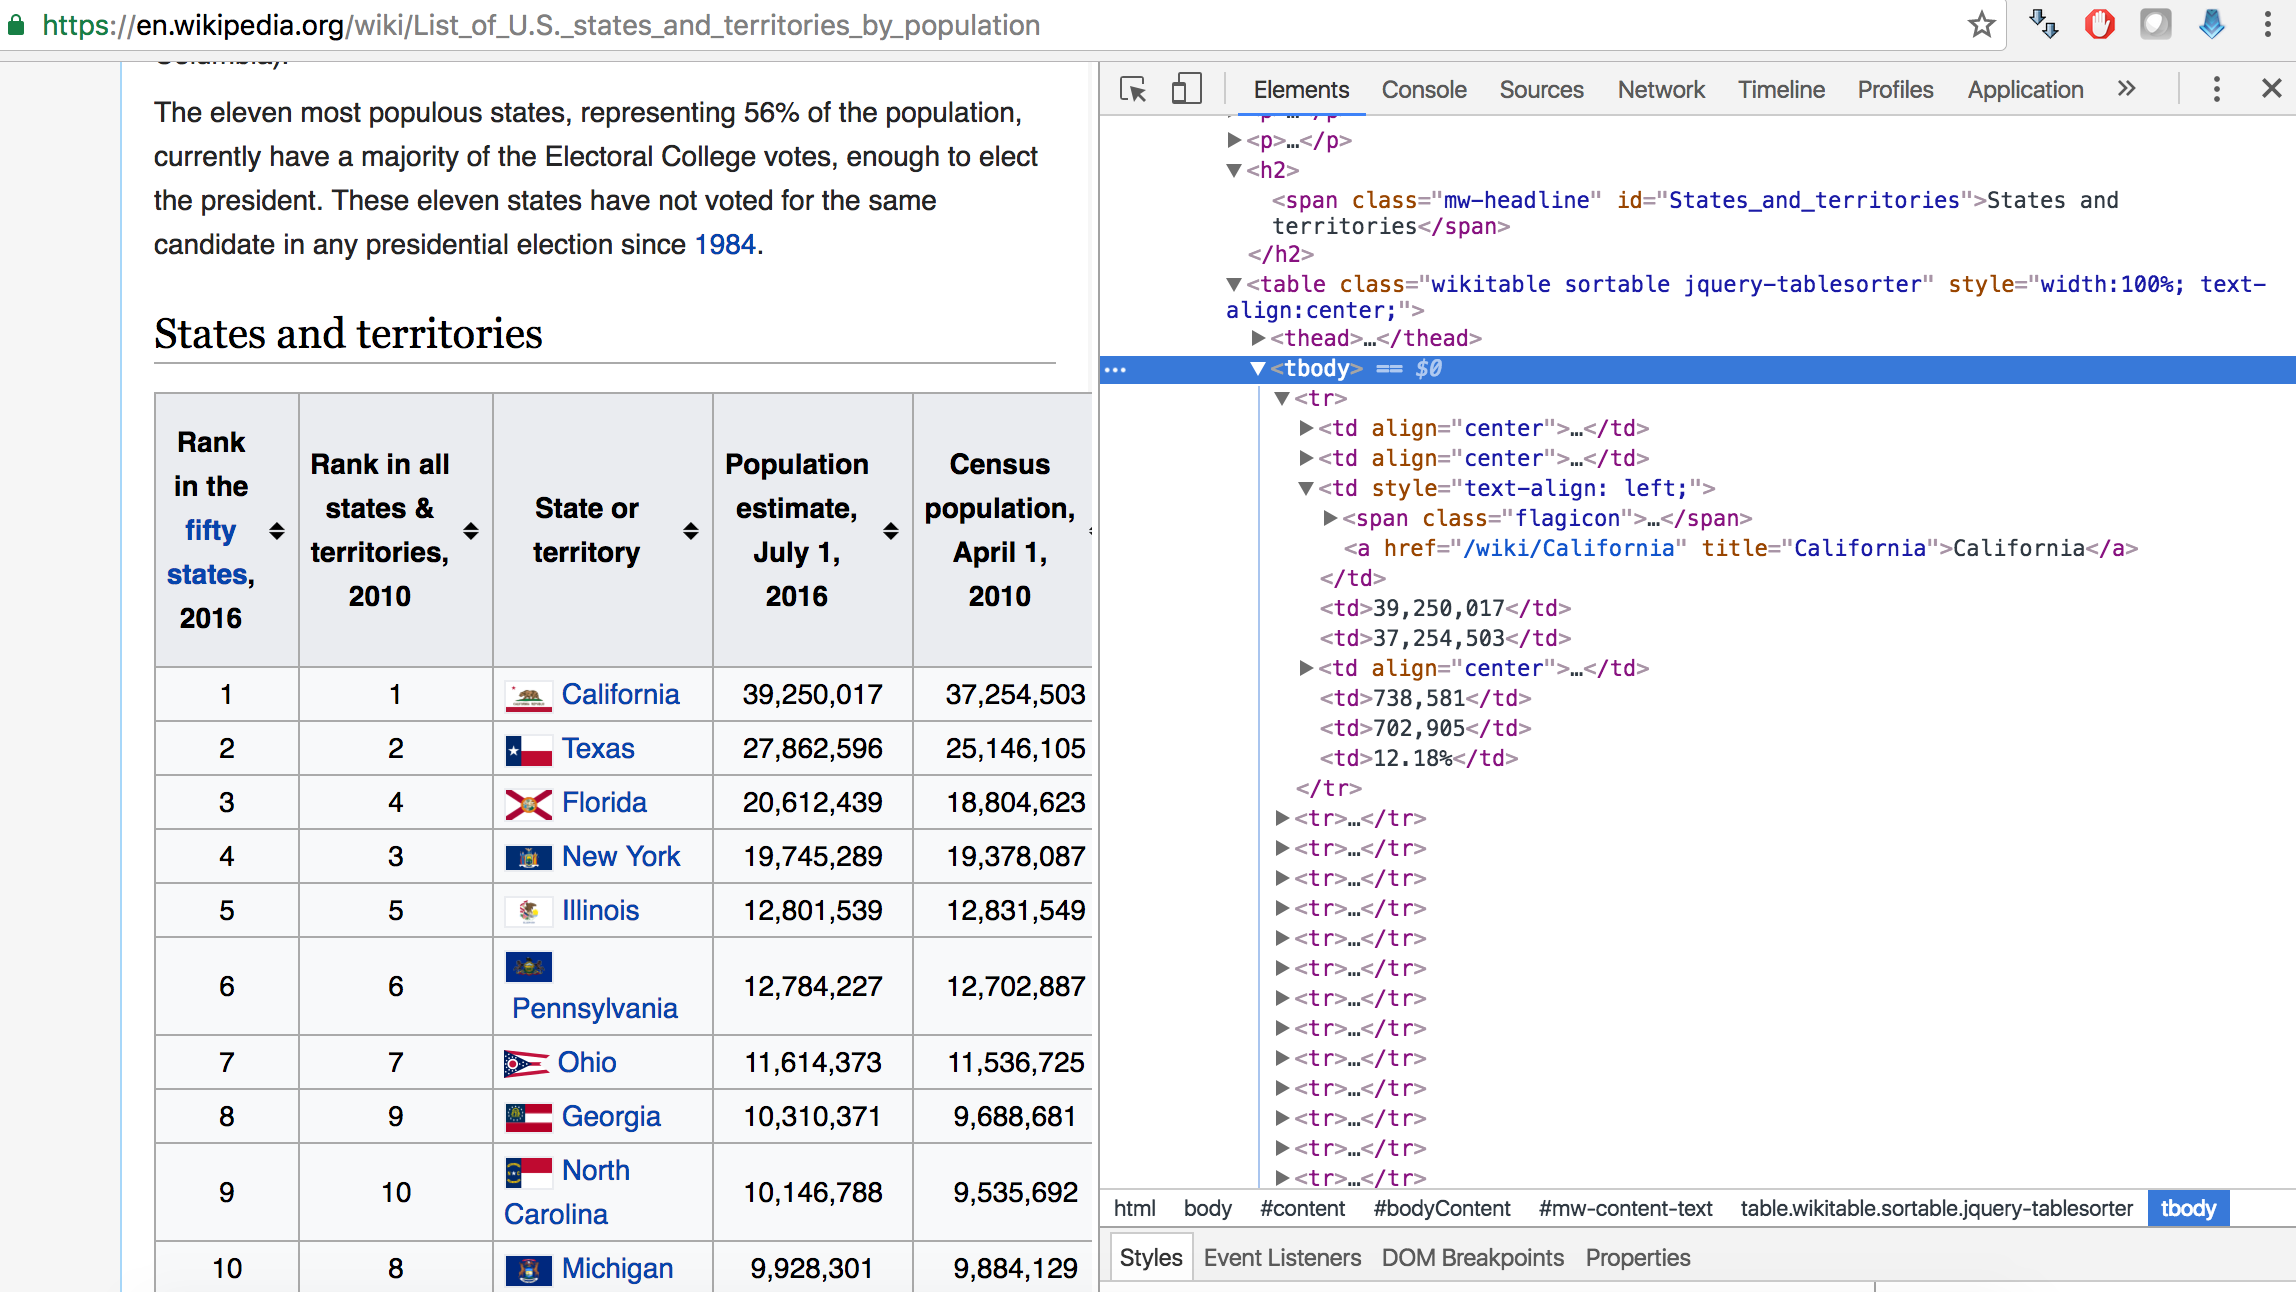
\includegraphics[scale=0.25]{figures/html-table-chrome.png}

\end{center}


$\Rightarrow$ Chrome's inspect element feature is very helpful in identifying the correct xpath to an element to be extracted (and to learn HTML while you are at it). 

\end{frame}
%%%%%%%%%%%%%%%%%%%%%%%%%%%%%%%%%%%%%%%%%%%%%%%%%%%%%%%%%%%%%%%%%%%%%%%%



%%%%%%%%%%%%%%%%%%%%%%%%%%%%%%%%%%%%%%%%%%%%%%%%%%%%%%%%%%
\begin{frame}[fragile]{Example: Extracting a HTML table the ``hard'' way}

\begin{knitrout}\tiny
\definecolor{shadecolor}{rgb}{0.969, 0.969, 0.969}\color{fgcolor}\begin{kframe}
\begin{alltt}
\hlstd{HTML}\hlkwb{<-}\hlkwd{readLines}\hlstd{(}\hlkwc{con}\hlstd{=}\hlstr{"https://en.wikipedia.org/wiki/List_of_U.S._states_and_territories_by_population"}\hlstd{)}
\hlcom{#subsetting}
\hlstd{HTML}\hlkwb{<-}\hlstd{HTML[}\hlkwd{grep}\hlstd{(}\hlstr{'<span class="mw-headline" id="States_and_territories">'}\hlstd{,}
                \hlstd{HTML)}\hlopt{:}\hlkwd{grep}\hlstd{(}\hlstr{'<span class="mw-headline" id="Summary_of_population_by_region">'}\hlstd{,HTML)]}

\hlkwd{head}\hlstd{(HTML)}
\end{alltt}
\begin{verbatim}
## [1] "<h2><span class=\"mw-headline\" id=\"States_and_territories\">States and territories</span></h2>"                                                        
## [2] "<table class=\"wikitable sortable\" style=\"width:100%; text-align:center;\">"                                                                           
## [3] "<tr style=\"vertical-align: top;\">"                                                                                                                     
## [4] "<th style=\"vertical-align: middle\">Rank in the <a href=\"/wiki/Fifty_States\" class=\"mw-redirect\" title=\"Fifty States\">fifty states</a>, 2016</th>"
## [5] "<th style=\"vertical-align: middle\">Rank in all states &amp; territories, 2010</th>"                                                                    
## [6] "<th style=\"width: 20%; vertical-align: middle\"><b>State or territory</b></th>"
\end{verbatim}
\begin{alltt}
\hlcom{#tr is a table-row}

\hlcom{#indices of start of new rows}
\hlkwd{grep}\hlstd{(}\hlstr{"<tr>"}\hlstd{,HTML)}
\end{alltt}
\begin{verbatim}
##  [1]  14  25  36  47  58  69  80  91 102 113 124 135 146 157 168 179 190 201 212 223 234
## [22] 245 256 267 278 289 300 311 322 344 355 366 377 388 399 410 421 432 443 454 465 476
## [43] 487 498 509 520 531 542 564 575
\end{verbatim}
\begin{alltt}
\hlstd{population}\hlkwb{<-}\hlkwd{lapply}\hlstd{(}\hlkwd{grep}\hlstd{(}\hlstr{"<tr>"}\hlstd{,HTML),} \hlkwa{function}\hlstd{(}\hlkwc{x}\hlstd{)} \hlkwd{gsub}\hlstd{(}\hlstr{"<.*?>"}\hlstd{,} \hlstr{""}\hlstd{, HTML[x}\hlopt{:}\hlstd{(x}\hlopt{+}\hlnum{10}\hlstd{)]))}
\hlstd{population}\hlkwb{<-}\hlkwd{lapply}\hlstd{(population,} \hlkwa{function}\hlstd{(}\hlkwc{x}\hlstd{) x[x}\hlopt{!=}\hlstr{""}\hlstd{])}

\hlstd{population}\hlkwb{<-}\hlkwd{do.call}\hlstd{(}\hlstr{"rbind"}\hlstd{, population)}
\hlkwd{class}\hlstd{(population)}
\end{alltt}
\begin{verbatim}
## [1] "matrix"
\end{verbatim}
\begin{alltt}
\hlkwd{head}\hlstd{(population)}
\end{alltt}
\begin{verbatim}
##      [,1]                    [,2]                    [,3]                 [,4]        
## [1,] "7000100000000000000♠1" "7000100000000000000♠1" "&#160;California"   "39,250,017"
## [2,] "7000200000000000000♠2" "7000200000000000000♠2" "&#160;Texas"        "27,862,596"
## [3,] "7000300000000000000♠3" "7000400000000000000♠4" "&#160;Florida"      "20,612,439"
## [4,] "7000400000000000000♠4" "7000300000000000000♠3" "&#160;New York"     "19,745,289"
## [5,] "7000500000000000000♠5" "7000500000000000000♠5" "&#160;Illinois"     "12,801,539"
## [6,] "7000600000000000000♠6" "7000600000000000000♠6" "&#160;Pennsylvania" "12,784,227"
##      [,5]         [,6]                     [,7]      [,8]      [,9]    
## [1,] "37,254,503" "7001530000000000000♠53" "738,581" "702,905" "12.15%"
## [2,] "25,146,105" "7001360000000000000♠36" "763,031" "698,487" "8.62%" 
## [3,] "18,804,623" "7001270000000000000♠27" "750,788" "696,345" "6.38%" 
## [4,] "19,378,087" "7001270000000000000♠27" "733,177" "717,707" "6.11%" 
## [5,] "12,831,549" "7001180000000000000♠18" "714,444" "712,813" "3.96%" 
## [6,] "12,702,887" "7001180000000000000♠18" "711,250" "705,688" "3.96%"
\end{verbatim}
\end{kframe}
\end{knitrout}

\end{frame}
%%%%%%%%%%%%%%%%%%%%%%%%%%%%%%%%%%%%%%%%%%%%%%%%%%%%%%%%%%%%%%%%%%%%%%%%


%%%%%%%%%%%%%%%%%%%%%%%%%%%%%%%%%%%%%%%%%%%%%%%%%%%%%%%%%%
\begin{frame}[fragile]{Example: Extracting data from a Wikipedia page table}


\begin{center}

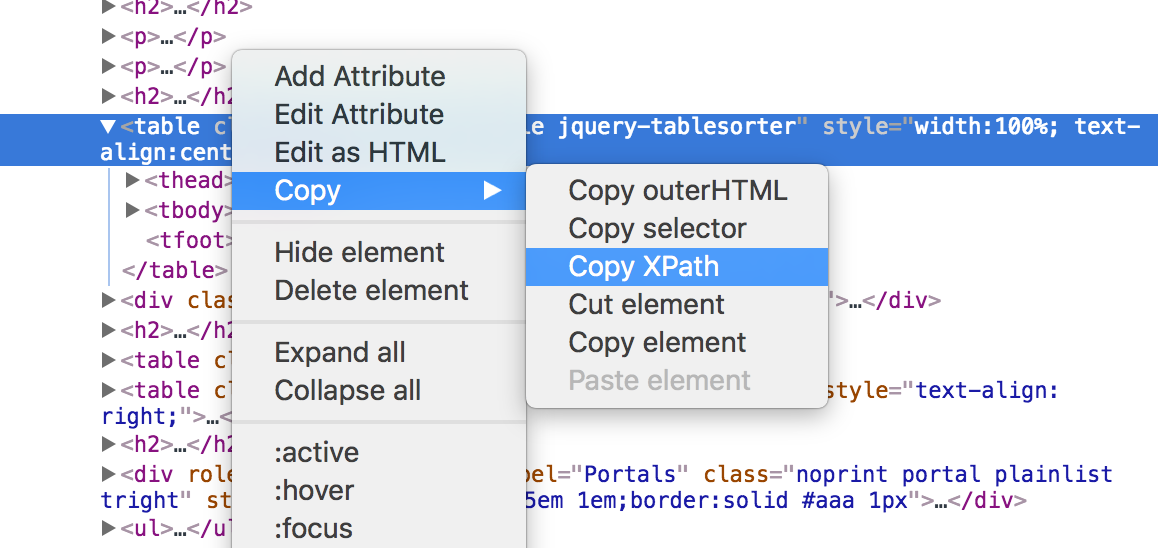
\includegraphics[scale=0.5]{figures/html-copy-xpath.png}

\end{center}


$\Rightarrow$ Chrome's inspect element feature is very helpful in identifying the correct xpath to an element to be extracted (and to learn HTML while you are at it). 

\end{frame}
%%%%%%%%%%%%%%%%%%%%%%%%%%%%%%%%%%%%%%%%%%%%%%%%%%%%%%%%%%%%%%%%%%%%%%%%



%%%%%%%%%%%%%%%%%%%%%%%%%%%%%%%%%%%%%%%%%%%%%%%%%%%%%%%%%%
\begin{frame}[fragile]{Example: Extracting a HTML table the ``easy'' way}
\begin{knitrout}\tiny
\definecolor{shadecolor}{rgb}{0.969, 0.969, 0.969}\color{fgcolor}\begin{kframe}
\begin{alltt}
\hlcom{#install.packages("rvest")}
\hlkwd{library}\hlstd{(}\hlstr{"rvest"}\hlstd{)}
\hlstd{url} \hlkwb{<-} \hlstr{"http://en.wikipedia.org/wiki/List_of_U.S._states_and_territories_by_population"}
\hlstd{population} \hlkwb{<-} \hlstd{url} \hlopt
  \hlkwd{read_html}\hlstd{()} \hlopt
  \hlkwd{html_nodes}\hlstd{(}\hlkwc{xpath}\hlstd{=}\hlstr{'//*[@id="mw-content-text"]/table[1]'}\hlstd{)} \hlopt
  \hlkwd{html_table}\hlstd{()}

\hlstd{population} \hlkwb{<-} \hlstd{population[[}\hlnum{1}\hlstd{]]}

\hlkwd{head}\hlstd{(population)}
\end{alltt}
\begin{verbatim}
##   Rank in the fifty states, 2016 Rank in all states & territories, 2010
## 1          7000100000000000000♠1                  7000100000000000000♠1
## 2          7000200000000000000♠2                  7000200000000000000♠2
## 3          7000300000000000000♠3                  7000400000000000000♠4
## 4          7000400000000000000♠4                  7000300000000000000♠3
## 5          7000500000000000000♠5                  7000500000000000000♠5
## 6          7000600000000000000♠6                  7000600000000000000♠6
##   State or territory Population estimate, July 1, 2016 Census population, April 1, 2010
## 1         California                        39,250,017                       37,254,503
## 2              Texas                        27,862,596                       25,146,105
## 3            Florida                        20,612,439                       18,804,623
## 4           New York                        19,745,289                       19,378,087
## 5           Illinois                        12,801,539                       12,831,549
## 6       Pennsylvania                        12,784,227                       12,702,887
##   Total seats in House of Representatives, 2013–2023 Estimated pop. per House seat, 2016
## 1                             7001530000000000000♠53                             738,581
## 2                             7001360000000000000♠36                             763,031
## 3                             7001270000000000000♠27                             750,788
## 4                             7001270000000000000♠27                             733,177
## 5                             7001180000000000000♠18                             714,444
## 6                             7001180000000000000♠18                             711,250
##   Census pop. per House seat, 2010 Percent of total U.S. pop., 2016[note 1]
## 1                          702,905                                   12.15%
## 2                          698,487                                    8.62%
## 3                          696,345                                    6.38%
## 4                          717,707                                    6.11%
## 5                          712,813                                    3.96%
## 6                          705,688                                    3.96%
\end{verbatim}
\end{kframe}
\end{knitrout}
\end{frame}
%%%%%%%%%%%%%%%%%%%%%%%%%%%%%%%%%%%%%%%%%%%%%%%%%%%%%%%%%%%%%%%%%%%%%%%%%




\section{API's}

%%%%%%%%%%%%%%%%%%%%%%%%%%%%%%%%%%%%%%%%%%%%%%%%%%%%%%%%%%
\begin{frame}[fragile]{APIs}

\begin{quote}
When used in the context of web development, an API is typically defined as a set of Hypertext Transfer Protocol (HTTP) request messages, along with a definition of the structure of response messages, which is usually in an Extensible Markup Language (XML) or JavaScript Object Notation (JSON) format.\\
\end{quote}
\begin{quote}
The practice of publishing APIs has allowed web communities to create an open architecture for sharing content and data between communities and applications. In this way, content that is created in one place can be dynamically posted and updated in multiple locations on the web
-Wikipedia
\end{quote}

$\Rightarrow$ many online servies and sites offer APIs, with some having dedicated R-packages (see Twitter and Facebook packages for R in a bit).
\end{frame}
%%%%%%%%%%%%%%%%%%%%%%%%%%%%%%%%%%%%%%%%%%%%date%%%%%%%%%%%%%%%%%%%%%%%%%%%%%


%%%%%%%%%%%%%%%%%%%%%%%%%%%%%%%%%%%%%%%%%%%%%%%%%%%%%%%%%%
\begin{frame}[fragile]{Lightweight JSON format to send and receive information}
JSON (Java Script Object Notation) is a very lightweight format to send and receive data, which is why it is typically preferred to XML for sending structured data to APIs.

\begin{knitrout}\tiny
\definecolor{shadecolor}{rgb}{0.969, 0.969, 0.969}\color{fgcolor}\begin{kframe}
\begin{alltt}
\hlcom{#download some wikipedia traffic statistics}
\hlstd{var}\hlkwb{=}\hlnum{201401}

\hlstd{url}\hlkwb{=}\hlkwd{paste}\hlstd{(}\hlstr{"http://stats.grok.se/json/en/"}\hlstd{,var,}\hlstr{"/Donald_Trump"}\hlstd{,}\hlkwc{sep}\hlstd{=}\hlstr{""}\hlstd{)}
\hlstd{raw.data} \hlkwb{<-} \hlkwd{readLines}\hlstd{(url,} \hlkwc{warn}\hlstd{=}\hlstr{"F"}\hlstd{)}

\hlcom{#raw JSON data}
\hlstd{raw.data}
\end{alltt}
\begin{verbatim}
## [1] "{\"daily_views\": {\"2014-01-15\": 3795, \"2014-01-14\": 3754, \"2014-01-17\": 3538, \"2014-01-16\": 3593, \"2014-01-11\": 4508, \"2014-01-10\": 4160, \"2014-01-13\": 3816, \"2014-01-12\": 4208, \"2014-01-19\": 3284, \"2014-01-18\": 3368, \"2014-01-28\": 3619, \"2014-01-29\": 3843, \"2014-01-20\": 4097, \"2014-01-21\": 4755, \"2014-01-22\": 9606, \"2014-01-23\": 5129, \"2014-01-24\": 3789, \"2014-01-25\": 3505, \"2014-01-26\": 3671, \"2014-01-27\": 3699, \"2014-01-06\": 0, \"2014-01-07\": 4660, \"2014-01-04\": 3745, \"2014-01-05\": 980, \"2014-01-02\": 4278, \"2014-01-03\": 3807, \"2014-01-01\": 2980, \"2014-01-08\": 4524, \"2014-01-09\": 4179, \"2014-01-31\": 3449, \"2014-01-30\": 3886}, \"project\": \"en\", \"month\": \"201401\", \"rank\": 4060, \"title\": \"Donald_Trump\"}"
\end{verbatim}
\begin{alltt}
\hlcom{#parsing JSON string into a list object}
\hlkwd{library}\hlstd{(RJSONIO)}
\hlstd{data}\hlkwb{<-}\hlkwd{fromJSON}\hlstd{(raw.data)}

\hlkwd{class}\hlstd{(data)}
\end{alltt}
\begin{verbatim}
## [1] "list"
\end{verbatim}
\begin{alltt}
\hlkwd{head}\hlstd{(data[[}\hlnum{1}\hlstd{]])}
\end{alltt}
\begin{verbatim}
## 2014-01-15 2014-01-14 2014-01-17 2014-01-16 2014-01-11 2014-01-10 
##       3795       3754       3538       3593       4508       4160
\end{verbatim}
\end{kframe}
\end{knitrout}

\end{frame}
%%%%%%%%%%%%%%%%%%%%%%%%%%%%%%%%%%%%%%%%%%%%%%%%%%%%%%%%%%%%%%%%%%%%%%%%%




%%%%%%%%%%%%%%%%%%%%%%%%%%%%%%%%%%%%%%%%%%%%%%%%%%%%%%%%%%
\begin{frame}[fragile]{Reading and Parsing JSON Data}
JSON is a very common format used by web services for sending and receiving data.
\begin{knitrout}\tiny
\definecolor{shadecolor}{rgb}{0.969, 0.969, 0.969}\color{fgcolor}\begin{kframe}
\begin{alltt}
\hlcom{#download some wikipedia traffic statistics}

\hlstd{datevector}\hlkwb{<-} \hlkwd{unlist}\hlstd{(}\hlkwd{lapply}\hlstd{(}\hlnum{2008}\hlopt{:}\hlnum{2016}\hlstd{,} \hlkwa{function}\hlstd{(}\hlkwc{x}\hlstd{)}
  \hlkwd{paste}\hlstd{(x,}\hlkwd{c}\hlstd{(}\hlstr{"01"}\hlstd{,}\hlstr{"02"}\hlstd{,}\hlstr{"03"}\hlstd{,}\hlstr{"04"}\hlstd{,}\hlstr{"05"}\hlstd{,}\hlstr{"06"}\hlstd{,}\hlstr{"07"}\hlstd{,}\hlstr{"08"}\hlstd{,}\hlstr{"09"}\hlstd{,}\hlstr{"10"}\hlstd{,}\hlstr{"11"}\hlstd{,}\hlstr{"12"}\hlstd{),}\hlkwc{sep}\hlstd{=}\hlstr{""}\hlstd{)))}

\hlkwd{head}\hlstd{(datevector)}
\end{alltt}
\begin{verbatim}
## [1] "200801" "200802" "200803" "200804" "200805" "200806"
\end{verbatim}
\begin{alltt}
\hlstd{datevector} \hlkwb{<-} \hlkwd{seq}\hlstd{(}\hlkwc{from} \hlstd{=} \hlkwd{as.POSIXct}\hlstd{(}\hlstr{"2008-01-01"}\hlstd{),} \hlkwc{to} \hlstd{=} \hlkwd{as.POSIXct}\hlstd{(}\hlstr{"2016-12-31"}\hlstd{),}
            \hlkwc{by} \hlstd{=} \hlstr{"months"}\hlstd{)}
\hlstd{datevector}\hlkwb{<-}\hlkwd{gsub}\hlstd{(}\hlstr{"-"}\hlstd{,}\hlstr{""}\hlstd{,}\hlkwd{substr}\hlstd{(datevector,} \hlnum{0}\hlstd{,}\hlnum{7}\hlstd{))}

\hlkwd{head}\hlstd{(datevector)}
\end{alltt}
\begin{verbatim}
## [1] "200801" "200802" "200803" "200804" "200805" "200806"
\end{verbatim}
\begin{alltt}
\hlcom{#this is not treated as character but as numeric as we create a sequence using the : operator}
\hlstd{datevector}\hlkwb{<-} \hlkwd{unlist}\hlstd{(}\hlkwd{lapply}\hlstd{(}\hlnum{2014}\hlopt{:}\hlnum{2016}\hlstd{,} \hlkwa{function}\hlstd{(}\hlkwc{x}\hlstd{)} \hlkwd{eval}\hlstd{(}\hlkwd{paste}\hlstd{(x,}\hlstr{"01"}\hlstd{,}\hlkwc{sep}\hlstd{=}\hlstr{""}\hlstd{)}\hlopt{:}\hlkwd{paste}\hlstd{(x,}\hlstr{"12"}\hlstd{,}\hlkwc{sep}\hlstd{=}\hlstr{""}\hlstd{))))}

\hlkwd{head}\hlstd{(datevector)}
\end{alltt}
\begin{verbatim}
## [1] 201401 201402 201403 201404 201405 201406
\end{verbatim}
\end{kframe}
\end{knitrout}

\end{frame}
%%%%%%%%%%%%%%%%%%%%%%%%%%%%%%%%%%%%%%%%%%%%%%%%%%%%%%%%%%%%%%%%%%%%%%%%%



%%%%%%%%%%%%%%%%%%%%%%%%%%%%%%%%%%%%%%%%%%%%%%%%%%%%%%%%%%
\begin{frame}[fragile]{Interest in Donald Trump on English Wikipedia over time}
\begin{knitrout}\tiny
\definecolor{shadecolor}{rgb}{0.969, 0.969, 0.969}\color{fgcolor}\begin{kframe}
\begin{alltt}
\hlcom{#download some wikipedia traffic statistics}

\hlstd{rd}\hlkwb{<-}\hlkwd{unlist}\hlstd{(}\hlkwd{lapply}\hlstd{(datevector,} \hlkwa{function}\hlstd{(}\hlkwc{x}\hlstd{)} \hlkwd{fromJSON}\hlstd{(}\hlkwd{readLines}\hlstd{(}
  \hlkwd{paste}\hlstd{(}\hlstr{"http://stats.grok.se/json/en/"}\hlstd{,x,}\hlstr{"/Donald_Trump"}\hlstd{,}\hlkwc{sep}\hlstd{=}\hlstr{""}\hlstd{) ))}\hlopt{$}\hlstd{daily_views))}

\hlstd{rd}\hlkwb{<-}\hlkwd{data.frame}\hlstd{(rd)}
\hlstd{rd}\hlopt{$}\hlstd{date}\hlkwb{<-}\hlkwd{strptime}\hlstd{(}\hlkwd{rownames}\hlstd{(rd),} \hlstr{"%Y-%m-%d"}\hlstd{)}
\hlstd{rd}\hlkwb{<-}\hlstd{rd[rd}\hlopt{>}\hlnum{0}\hlstd{,]}
\hlstd{rd}\hlkwb{<-}\hlstd{rd[}\hlkwd{order}\hlstd{(rd}\hlopt{$}\hlstd{date),]}
\hlkwd{plot}\hlstd{(rd}\hlopt{$}\hlstd{date,} \hlkwd{log}\hlstd{(rd}\hlopt{$}\hlstd{rd}\hlopt{+}\hlnum{1}\hlstd{),} \hlkwc{type}\hlstd{=}\hlstr{"l"}\hlstd{)}
\end{alltt}
\end{kframe}

{\centering 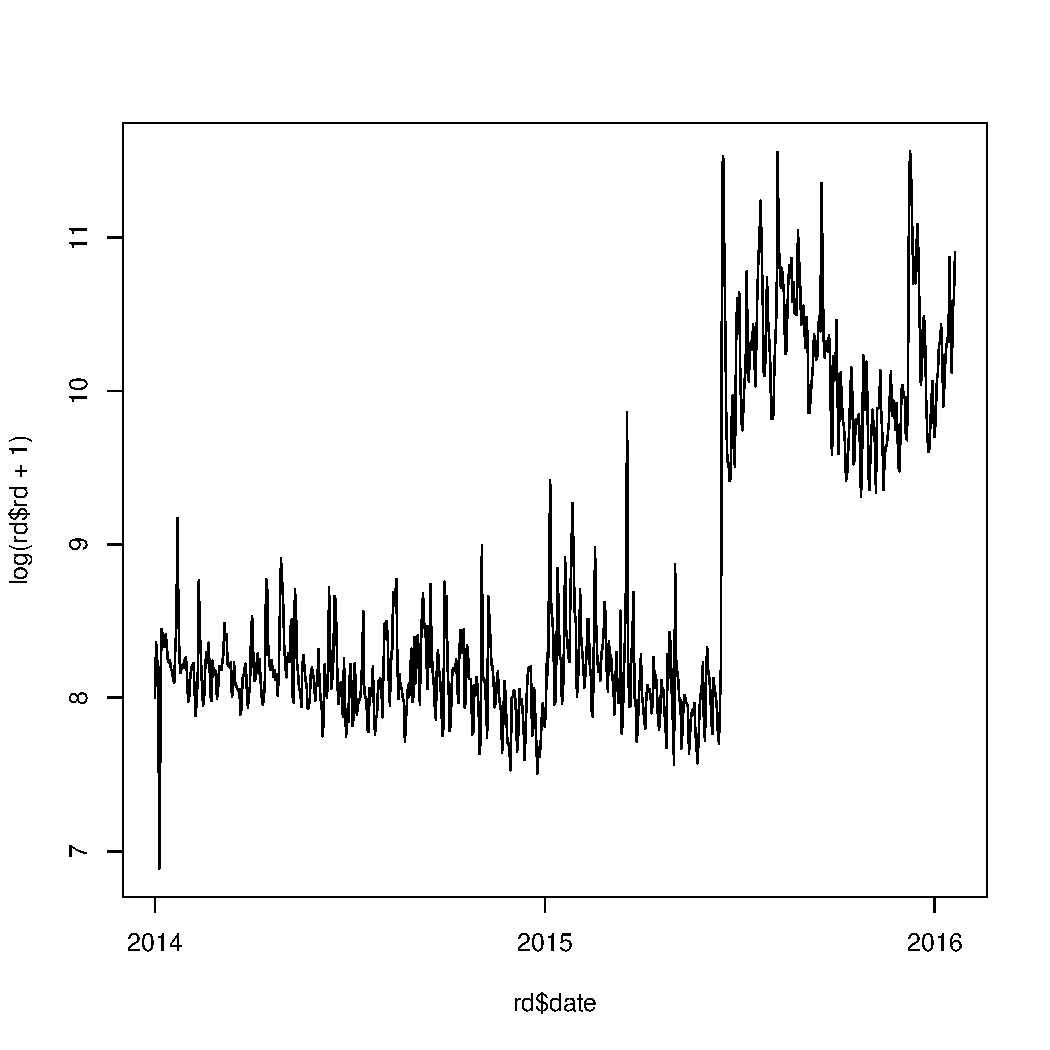
\includegraphics[width=2.4in]{figures/knitr-readingtext7-1} 

}



\end{knitrout}

\end{frame}
%%%%%%%%%%%%%%%%%%%%%%%%%%%%%%%%%%%%%%%%%%%%%%%%%%%%%%%%%%%%%%%%%%%%%%%%%


%%%%%%%%%%%%%%%%%%%%%%%%%%%%%%%%%%%%%%%%%%%%%%%%%%%%%%%%%%
\begin{frame}[fragile]{Social Media API's}

\begin{itemize}

\item All big social media sites  - Facebook and Twitter - provide an API that allows access to their data. \smallskip

\item API's can either be anonymous or require authentication  \smallskip

\item API's tend to communicate through JSON data objects.\smallskip

\item Calls to APIs are sent through HTTP, so you can just call them using your browser\smallskip

\item API calls are just "complicated URLs".\smallskip

\item For our purposes, we will just highlight existing packages implemented for $R$ to access social media data from Facebook and Twitter.

\end{itemize}
\end{frame}
%%%%%%%%%%%%%%%%%%%%%%%%%%%%%%%%%%%%%%%%%%%%%%%%%%%%%%%%%%%%%%%%%%%%%%%%%


%%%%%%%%%%%%%%%%%%%%%%%%%%%%%%%%%%%%%%%%%%%%%%%%%%%%%%%%%%
\begin{frame}[fragile]{Types of Requests}

\begin{quote}
\code{GET} requests a representation of the specified resource. Note that GET should not be used for operations that cause side-effects, such as using it for taking actions in web applications. One reason for this is that GET may be used arbitrarily by robots or crawlers, which should not need to consider the side effects that a request should cause. 
\end{quote}

\begin{quote}
\code{POST} submits data to be processed (e.g., from an HTML form) to the identified resource. The data is included in the body of the request. This may result in the creation of a new resource or the updates of existing resources or both.
we use ‘get’ for scraping, ‘post’ is more complicated. Use it to navigate logins, popups, etc.
\end{quote}
\end{frame}
%%%%%%%%%%%%%%%%%%%%%%%%%%%%%%%%%%%%%%%%%%%%%%%%%%%%%%%%%%%%%%%%%%%%%%%%%


%%%%%%%%%%%%%%%%%%%%%%%%%%%%%%%%%%%%%%%%%%%%%%%%%%%%%%%%%%
\begin{frame}[fragile]{Named Entity Recognition via Web API}

\begin{knitrout}\tiny
\definecolor{shadecolor}{rgb}{0.969, 0.969, 0.969}\color{fgcolor}\begin{kframe}
\begin{alltt}
 \hlstd{url} \hlkwb{<-} \hlstr{'http://www.huffingtonpost.com/entry/house-republicans-ethics_us_586bdb14e4b0de3a08f99e66?6ztihpvi'}
\hlstd{api} \hlkwb{<-} \hlstr{'http://juicer.herokuapp.com/api/article?url='}
\hlstd{target} \hlkwb{<-} \hlkwd{paste}\hlstd{(api,url,}\hlkwc{sep}\hlstd{=}\hlstr{""}\hlstd{)}

\hlstd{raw.data} \hlkwb{<-} \hlkwd{readLines}\hlstd{(target,} \hlkwc{warn}\hlstd{=}\hlstr{"F"}\hlstd{)}

\hlstd{rd} \hlkwb{<-} \hlkwd{fromJSON}\hlstd{(raw.data)}
\hlstd{dat} \hlkwb{<-} \hlstd{rd}\hlopt{$}\hlstd{article}

\hlstd{ENTITIES}\hlkwb{<-}\hlkwd{data.frame}\hlstd{(}\hlkwd{do.call}\hlstd{(}\hlstr{"rbind"}\hlstd{, dat}\hlopt{$}\hlstd{entities))}

\hlstd{ENTITIES[}\hlnum{1}\hlopt{:}\hlnum{10}\hlstd{,]}
\end{alltt}
\begin{verbatim}
##            type                                                      text frequency
## 1        Person                                                     Trump         1
## 2  Organization Campaign for Accountability , Citizens for Responsibility         1
## 3        Person                                              Nancy Pelosi         1
## 4  Organization                                                     House         3
## 5  Organization                                           People 's House         1
## 6        Person                                                 Goodlatte         1
## 7      Location                                                Washington         2
## 8        Person                                                 Paul Ryan         1
## 9      Location                                                WASHINGTON         1
## 10       Person                                                    Pelosi         1
\end{verbatim}
\end{kframe}
\end{knitrout}

$\Rightarrow$ this works off the Stanford NLP NER module, which we will also directly use in R. 
\end{frame}
%%%%%%%%%%%%%%%%%%%%%%%%%%%%%%%%%%%%%%%%%%%%%%%%%%%%%%%%%%%%%%%%%%%%%%%%%





%%%%%%%%%%%%%%%%%%%%%%%%%%%%%%%%%%%%%%%%%%%%%%%%%%%%%%%%%%
\begin{frame}[fragile]{Social Media}


\begin{figure}[htb]
\begin{center}
$%
\begin{array}{cc}
\includegraphics[scale=.6]<1>{figures/social-media.png}
\includegraphics[scale=.4]<2>{figures/social-media-trump.png} &\includegraphics[scale=.4]<2>{figures/social-media-warren.png} 
\end{array}%
$%
\end{center}
\end{figure}

\end{frame}
%%%%%%%%%%%%%%%%%%%%%%%%%%%%%%%%%%%%%%%%%%%%%%%%%%%%%%%%%%%%%%%%%%%%%%%%%



%%%%%%%%%%%%%%%%%%%%%%%%%%%%%%%%%%%%%%%%%%%%%%%%%%%%%%%%%%
\begin{frame}[fragile]{Why working with Social Media data?}

Social media is changing the way politicians, (government) organizations and corporations are interacting with ther electorate, stakeholders and customers. \smallskip

Questions that arise from reasearch are not constrained but may include...\smallskip
\begin{itemize}

\item How do politicians engage with their electorate through social media?\smallskip

\item Does direct communication via social media replace reliance on other media sources?\smallskip

\item Does social media allow for a more effective monitoring of elected officials? \smallskip


\end{itemize}

And there are likely a lot more... most social media data takes form of texts or tweets, so how can we get this data to work with?

\end{frame}
%%%%%%%%%%%%%%%%%%%%%%%%%%%%%%%%%%%%%%%%%%%%%%%%%%%%%%%%%%%%%%%%%%%%%%%%%


%%%%%%%%%%%%%%%%%%%%%%%%%%%%%%%%%%%%%%%%%%%%%%%%%%%%%%%%%%
\begin{frame}[fragile]{\code{TwitteR}}

\begin{itemize}

\item \code{TwitteR} package allows for basic Twitter scraping functionality. \smallskip

\item Need to create an access token to verify identity of requests (and to limit usage) \smallskip

\item \code{TwitteR} package handles authentification process and has core functionality to ...

\begin{itemize}

\item Scrape tweets pertaining to individual hashtags
\item Scrape timelines of Twitter users
\item get data on follower network structure (who follows whom)
\end{itemize}


\includegraphics[scale=.25]{figures/twitter-register.png}
\end{itemize}
\end{frame}
%%%%%%%%%%%%%%%%%%%%%%%%%%%%%%%%%%%%%%%%%%%%%%%%%%%%%%%%%%%%%%%%%%%%%%%%%




%%%%%%%%%%%%%%%%%%%%%%%%%%%%%%%%%%%%%%%%%%%%%%%%%%%%%%%%%%
\begin{frame}[fragile]{Sourcing Twitter data: Hash-tag level}
\begin{knitrout}\tiny
\definecolor{shadecolor}{rgb}{0.969, 0.969, 0.969}\color{fgcolor}\begin{kframe}
\begin{alltt}
\hlkwd{library}\hlstd{(twitteR)}
\hlcom{#setup_twitter_oauth(consumer_key, consumer_secret, access_token=NULL, access_secret=NULL)}
\hlkwd{set.seed}\hlstd{(}\hlnum{12122016}\hlstd{)}
\hlstd{tw} \hlkwb{=} \hlkwd{searchTwitter}\hlstd{(}\hlstr{'#Brexit'}\hlstd{,} \hlkwc{n} \hlstd{=} \hlnum{500}\hlstd{,} \hlkwc{since} \hlstd{=} \hlstr{'2016-12-12'}\hlstd{,} \hlkwc{lang}\hlstd{=}\hlstr{"en"}\hlstd{)}
\hlstd{tw.df}\hlkwb{<-} \hlkwd{data.table}\hlstd{(}\hlkwd{twListToDF}\hlstd{(tw))}
\hlkwd{strwrap}\hlstd{(}\hlkwd{head}\hlstd{(tw.df}\hlopt{$}\hlstd{text))}
\end{alltt}
\begin{verbatim}
##  [1] "RT @Aon_UK: Aon has launched #Brexit Navigator. Watch the video and request your" 
##  [2] "online demo here https://t.co/N4vtJjOpAI https://t.co/uJ7h…"                      
##  [3] "RT @HighRise_movie: What does #HighRise say about #Brexit?"                       
##  [4] "https://t.co/efQgGGF0zm via @engagingculture https://t.co/Y7tQjQ2yA4"             
##  [5] "RT @UKIPNFKN: Brexit transition: the problem that haunted Rogers via @FT #Brexit" 
##  [6] "#Brussels https://t.co/oD5T1gNsah"                                                
##  [7] "RT @david_bychkov: RT_com: ‘Juvenile delinquent, has no clue about #Brexit’ - EU" 
##  [8] "commissioner blasts Nigel Farage https://t.co/rwEXSIIp9w"                         
##  [9] "RT @SMTuffy: Consider this your official warning: \"Jenga\" is about to enter the"
## [10] "#Brexit lexicon https://t.co/3GEKKIUFKp"                                          
## [11] "RT @UKHouseofLords: #LordsQs start as peers press govt on impact of #Brexit on"   
## [12] "economy of North East England, watch live https://t.co/A5dQ6…"
\end{verbatim}
\begin{alltt}
\hlkwd{save}\hlstd{(tw.df,} \hlkwc{file}\hlstd{=}\hlstr{"../../Data/brexittweets.rdata"}\hlstd{)}
\end{alltt}
\end{kframe}
\end{knitrout}

\end{frame}
%%%%%%%%%%%%%%%%%%%%%%%%%%%%%%%%%%%%%%%%%%%%%%%%%%%%%%%%%%%%%%%%%%%%%%%%%

\begin{frame}[fragile]{Sourcing Twitter data: Individual user level}
\begin{knitrout}\tiny
\definecolor{shadecolor}{rgb}{0.969, 0.969, 0.969}\color{fgcolor}\begin{kframe}
\begin{alltt}
\hlkwd{library}\hlstd{(twitteR)}
\hlcom{#setup_twitter_oauth(consumer_key, consumer_secret, access_token=NULL, access_secret=NULL)}
\hlkwd{set.seed}\hlstd{(}\hlnum{12122016}\hlstd{)}
\hlstd{tw.user} \hlkwb{=} \hlkwd{userTimeline}\hlstd{(}\hlstr{'Nigel_Farage'}\hlstd{,}\hlkwc{n}\hlstd{=}\hlnum{500}\hlstd{)}
\hlstd{tw.user.df}\hlkwb{<-} \hlkwd{data.table}\hlstd{(}\hlkwd{twListToDF}\hlstd{(tw.user))}
\hlkwd{strwrap}\hlstd{(}\hlkwd{head}\hlstd{(tw.user.df}\hlopt{$}\hlstd{text))}
\end{alltt}
\begin{verbatim}
##  [1] "I don't think @Theresa_May has the flair, excitement or vision to lead this"     
##  [2] "country into its new Brexit chapter. https://t.co/wm84McM50L"                    
##  [3] "If you thought the PM was confusing over the single market, Corbyn's position on"
##  [4] "immigration is even more intriguing https://t.co/4cZ5GzqA1o"                     
##  [5] "Pleased to hear @SenBobCorker so positive about UK-US trade deal"                
##  [6] "https://t.co/Pa6E3PwdcU"                                                         
##  [7] "My brand new show starts on @LBC at 7pm #FarageOnLBC https://t.co/fvVgZlNfTS"    
##  [8] "I've arrived at @LBC for The Nigel Farage Show. Watch live on their Facebook"    
##  [9] "page from 7pm! #FarageOnLBC https://t.co/uXqARnpWCV"                             
## [10] "More reassuring words from Mrs May on Sky this morning, but same line for"       
## [11] "several months now. When will it convert into action?"
\end{verbatim}
\begin{alltt}
\hlkwd{save}\hlstd{(tw.user.df,} \hlkwc{file}\hlstd{=}\hlstr{"../../Data/nigelstweets.rdata"}\hlstd{)}
\end{alltt}
\end{kframe}
\end{knitrout}

\end{frame}
%%%%%%%%%%%%%%%%%%%%%%%%%%%%%%%%%%%%%%%%%%%%%%%%%%%%%%%%%%








%%%%%%%%%%%%%%%%%%%%%%%%%%%%%%%%%%%%%%%%%%%%%%%%%%%%%%%%%%
\begin{frame}[fragile]{\code{Rfacebook}}

\begin{itemize}

\item \code{Rfacebook} package allows for very basic access to facebook post data on public profile pages. \smallskip

\item This can be useful to extract data on posting activity by politicians, in particular, regarding the messages sent. \smallskip

\item Authentification for \code{rFacebook} is more involved

\item Simple access token can be generated, but its only valid for two hours

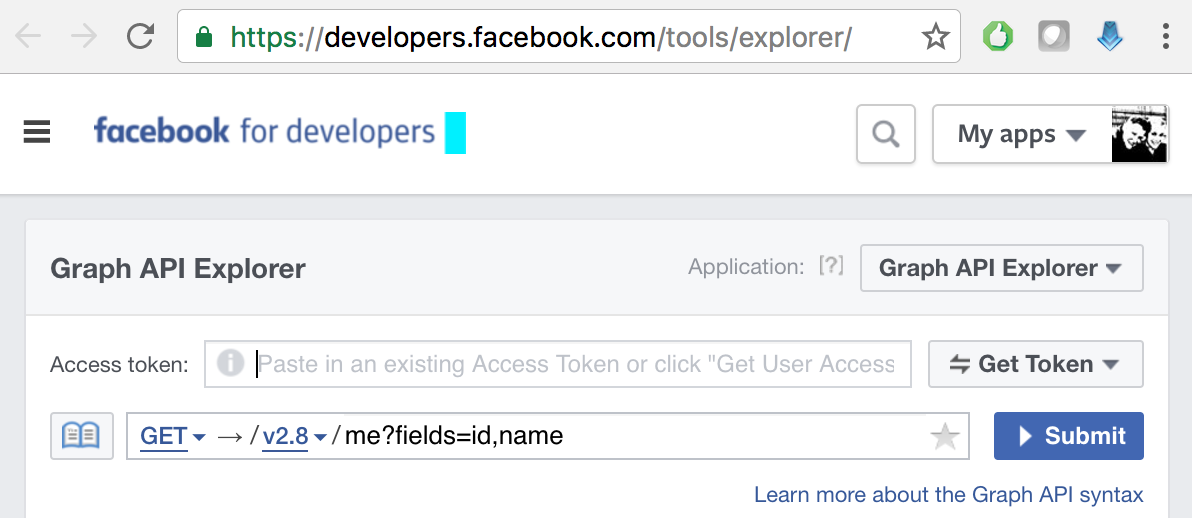
\includegraphics[scale=.35]{figures/fb-temporary-access-token.png}
\end{itemize}
\end{frame}
%%%%%%%%%%%%%%%%%%%%%%%%%%%%%%%%%%%%%%%%%%%%%%%%%%%%%%%%%%%%%%%%%%%%%%%%%


%%%%%%%%%%%%%%%%%%%%%%%%%%%%%%%%%%%%%%%%%%%%%%%%%%%%%%%%%%
\begin{frame}[fragile]{Creating a non-temporary authentification token for \code{Rfacebook}}

\begin{itemize}

\item To create a token that is valid for around two month period, you need to follow two steps.

\item Create a new app on \url{developers.facebook.com/apps/}, note down APP ID and APP SECRET and register the URL \url{http://localhost:1410/} under Settings - Basic - New platform
\end{itemize}
\begin{center}
\includegraphics[scale=0.25]<1>{figures/fb-newapp.png}
\includegraphics[scale=0.2]<2>{figures/fb-add-platform.png}
\includegraphics[scale=0.2]<3>{figures/fb-add-website.png}
\end{center}
\end{frame}
%%%%%%%%%%%%%%%%%%%%%%%%%%%%%%%%%%%%%%%%%%%%%%%%%%%%%%%%%%%%%%%%%%%%%%%%%


%%%%%%%%%%%%%%%%%%%%%%%%%%%%%%%%%%%%%%%%%%%%%%%%%%%%%%%%%%
\begin{frame}[fragile]{Creating a non-temporary authentification token for \code{Rfacebook}}

\begin{itemize}
\item In R, type the following lines
\begin{knitrout}\tiny
\definecolor{shadecolor}{rgb}{0.969, 0.969, 0.969}\color{fgcolor}\begin{kframe}
\begin{alltt}
\hlkwd{require}\hlstd{(}\hlstr{"Rfacebook"}\hlstd{)}
\hlstd{fb_oauth} \hlkwb{<-} \hlkwd{fbOAuth}\hlstd{(}\hlkwc{app_id}\hlstd{=}\hlstr{"APPNUMBER"}\hlstd{,} \hlkwc{app_secret}\hlstd{=}\hlstr{"APPSECRET"}\hlstd{,}\hlkwc{extended_permissions} \hlstd{=} \hlnum{TRUE}\hlstd{)}
\hlcom{#should open a browser window and facebook page to grant accesss to the app.}

\hlcom{#save the token for later reuse}
\hlkwd{save}\hlstd{(fb_oauth,} \hlkwc{file}\hlstd{=}\hlstr{"fb_oauth.rdata"}\hlstd{)}

\hlkwd{load}\hlstd{(}\hlkwc{file}\hlstd{=}\hlstr{"fb_oauth.rdata"}\hlstd{)}
\end{alltt}
\end{kframe}
\end{knitrout}
\item This should open a browser window in which you are asked to grant permission to the App to login via your account.

\item You should then save the access token and load it, so that you do not need to repeat this process each time you run a script.

\end{itemize}
\end{frame}
%%%%%%%%%%%%%%%%%%%%%%%%%%%%%%%%%%%%%%%%%%%%%%%%%%%%%%%%%%%%%%%%%%%%%%%%%

%%%%%%%%%%%%%%%%%%%%%%%%%%%%%%%%%%%%%%%%%%%%%%%%%%%%%%%%%%%%%%%%%%%%%%%%%
\begin{frame}[fragile]{Sourcing Facebook-page data}
\begin{knitrout}\tiny
\definecolor{shadecolor}{rgb}{0.969, 0.969, 0.969}\color{fgcolor}\begin{kframe}
\begin{alltt}
\hlkwd{require}\hlstd{(}\hlstr{"Rfacebook"}\hlstd{)}

\hlstd{me} \hlkwb{<-} \hlkwd{getUsers}\hlstd{(}\hlstr{"me"}\hlstd{, fb_oauth,} \hlkwc{private_info}\hlstd{=}\hlnum{TRUE}\hlstd{)}
\hlstd{me}\hlopt{$}\hlstd{name} \hlcom{# my name}
\end{alltt}
\begin{verbatim}
## [1] "Thiemo Fetzer"
\end{verbatim}
\begin{alltt}
\hlstd{page} \hlkwb{<-} \hlkwd{getPage}\hlstd{(}\hlstr{"barackobama"}\hlstd{, fb_oauth,} \hlkwc{n} \hlstd{=} \hlnum{100}\hlstd{)}
\end{alltt}
\begin{verbatim}
## 25 posts 50 posts 75 posts 100 posts
\end{verbatim}
\begin{alltt}
\hlkwd{strwrap}\hlstd{(}\hlkwd{head}\hlstd{(page}\hlopt{$}\hlstd{message))}
\end{alltt}
\begin{verbatim}
##  [1] "\"Our goal wasn't just to make sure more people have coverage—it was to make sure"
##  [2] "more people have better coverage.\" —President Obama"                             
##  [3] "NA"                                                                               
##  [4] "Today marks a crucial step forward in the fight against climate change, as the"   
##  [5] "historic Paris Climate Agreement officially enters into force."                   
##  [6] ""                                                                                 
##  [7] "Let's keep pushing for progress."                                                 
##  [8] "The economic progress we're making is undeniable—and it's up to all of us to"     
##  [9] "keep building an economy that works for all Americans."                           
## [10] "Obamacare was designed on the principle that health care coverage that's"         
## [11] "affordable, accessible to all, and free from discrimination should be a right,"   
## [12] "not a privilege. We can't afford to let opponents roll that back."                
## [13] "Millions of Americans are benefiting from Obamacare."
\end{verbatim}
\end{kframe}
\end{knitrout}

\end{frame}
%%%%%%%%%%%%%%%%%%%%%%%%%%%%%%%%%%%%%%%%%%%%%%%%%%%%%%%%%%


\section{Open Government API's and R packages}



%%%%%%%%%%%%%%%%%%%%%%%%%%%%%%%%%%%%%%%%%%%%%%%%%%%%%%%%%%
\begin{frame}[fragile]{Some R-accessible open government type API's}

\begin{center}

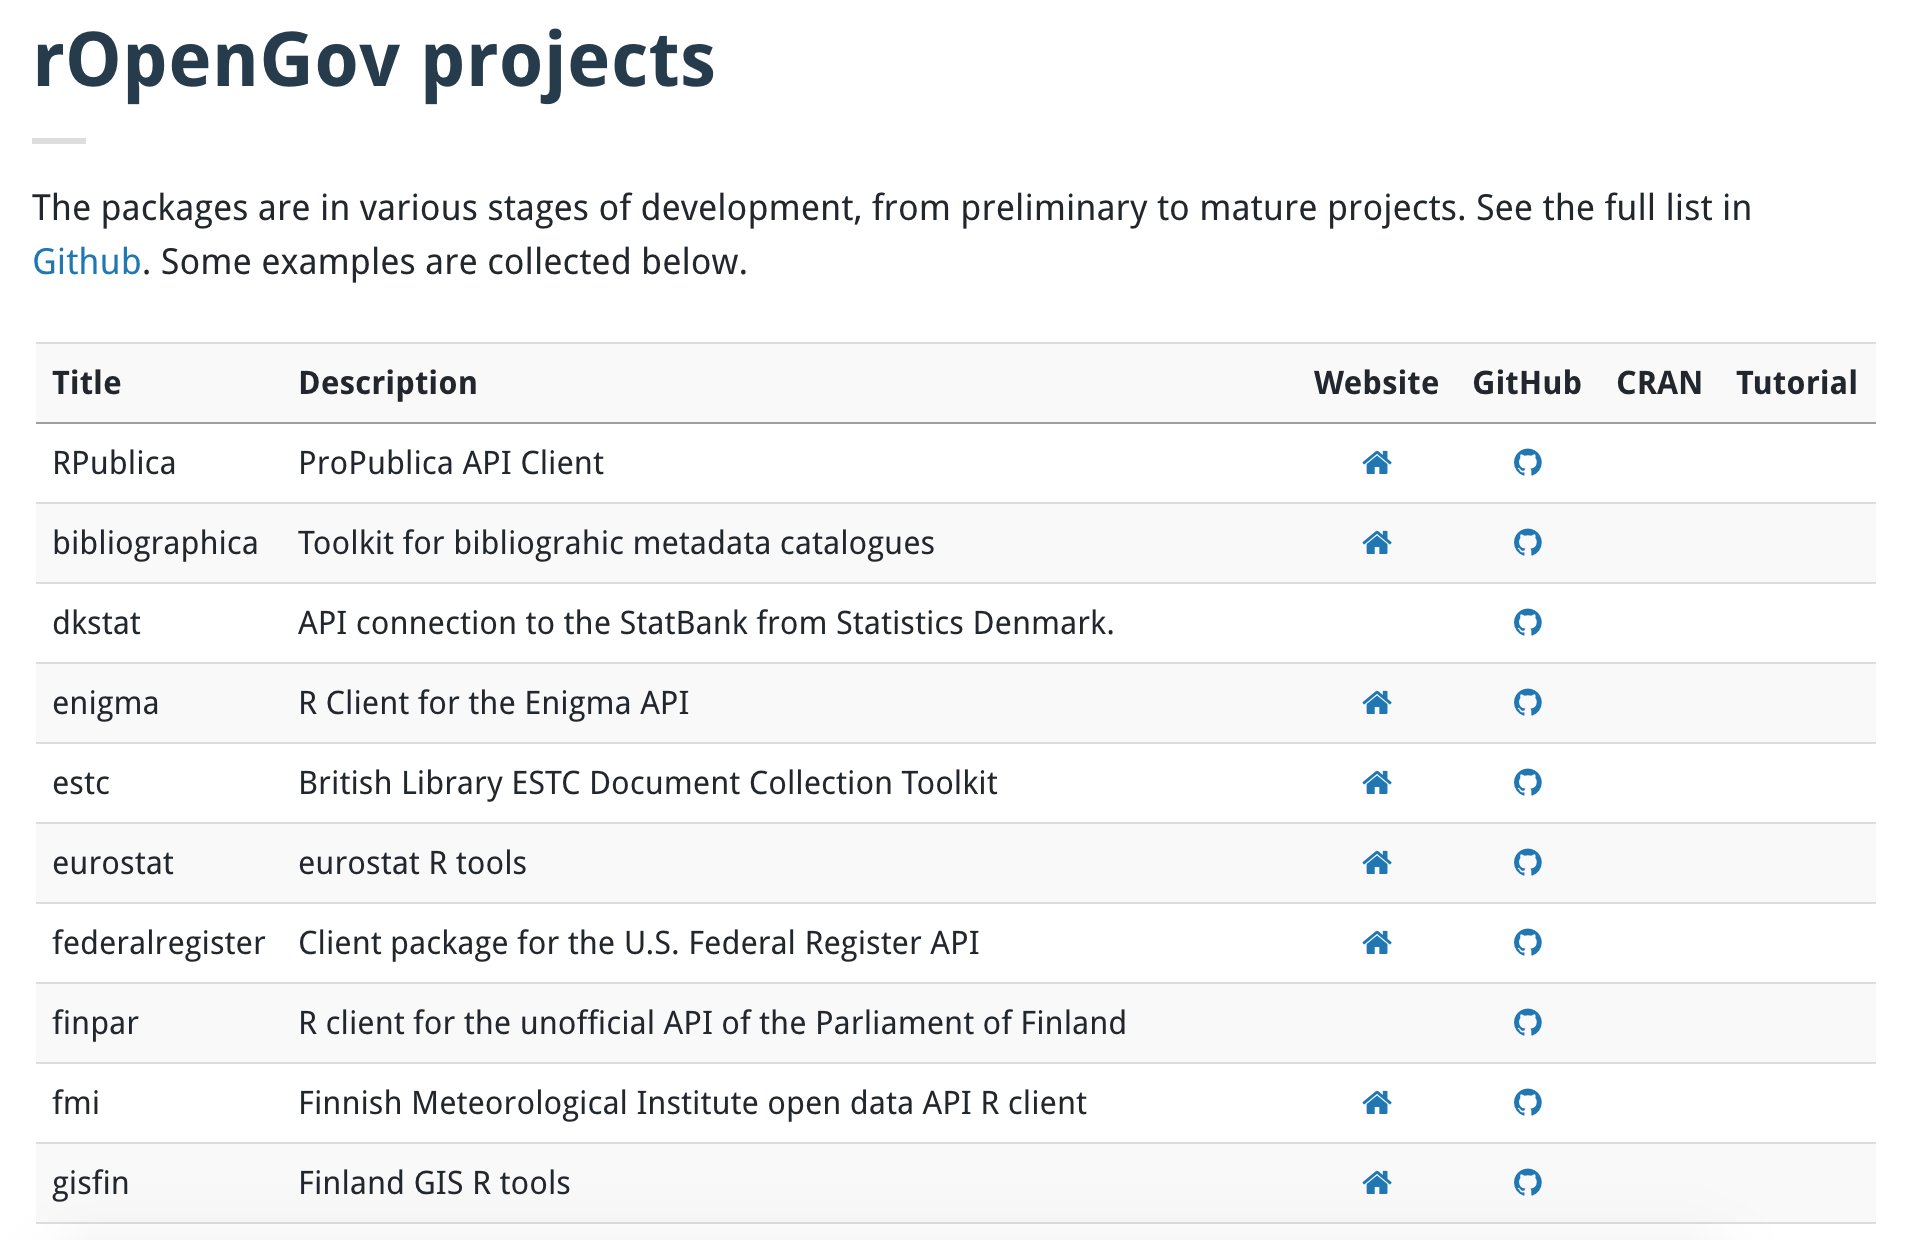
\includegraphics[scale=0.5]{figures/ropengov.png}

\end{center}
\end{frame}
%%%%%%%%%%%%%%%%%%%%%%%%%%%%%%%%%%%%%%%%%%%%%%%%%%%%%%%%%%%%%%%%%%%%%%%%%



%%%%%%%%%%%%%%%%%%%%%%%%%%%%%%%%%%%%%%%%%%%%%%%%%%%%%%%%%%
\begin{frame}[fragile]{Political Party \code{manifestoR} database for R}

\begin{quote}
ManifestoR is a free package for the open source statistical software R. It provides access to coded election programmes from the Manifesto Corpus and to the Manifesto Project's Main Dataset.
\end{quote}


Available via 

\begin{knitrout}\tiny
\definecolor{shadecolor}{rgb}{0.969, 0.969, 0.969}\color{fgcolor}\begin{kframe}
\begin{alltt}
\hlkwd{install.packages}\hlstd{(}\hlstr{"manifestoR"}\hlstd{)}
\hlkwd{library}\hlstd{(manifestoR)}
\end{alltt}
\end{kframe}
\end{knitrout}

Need to create an account and register for an API key on

\url{https://manifestoproject.wzb.eu/information/documents/manifestoR}

$\Rightarrow$ may be useful to study raising Euro(pe)-skepticism...

\end{frame}
%%%%%%%%%%%%%%%%%%%%%%%%%%%%%%%%%%%%%%%%%%%%%%%%%%%%%%%%%%%%%%%%%%%%%%%%%



%%%%%%%%%%%%%%%%%%%%%%%%%%%%%%%%%%%%%%%%%%%%%%%%%%%%%%%%%%
\begin{frame}[fragile]{Political Party \code{manifestoR} database for R}

\begin{knitrout}\tiny
\definecolor{shadecolor}{rgb}{0.969, 0.969, 0.969}\color{fgcolor}\begin{kframe}
\begin{alltt}
\hlkwd{install.packages}\hlstd{(}\hlstr{"manifestoR"}\hlstd{)}
\hlkwd{library}\hlstd{(manifestoR)}
\end{alltt}
\end{kframe}
\end{knitrout}

Print out some manifesto information.

\end{frame}
%%%%%%%%%%%%%%%%%%%%%%%%%%%%%%%%%%%%%%%%%%%%%%%%%%%%%%%%%%%%%%%%%%%%%%%%%


%%%%%%%%%%%%%%%%%%%%%%%%%%%%%%%%%%%%%%%%%%%%%%%%%%%%%%%%%%
\begin{frame}[fragile]{\code{rsunlight} package for R}

\textbf{CURRENTLY NOT FUNCTIONAL DUE TO TRANSFER TO POLITICO}

\begin{quote}
The Sunlight Foundation is an American 501 nonpartisan, nonprofit organization that advocates for open government.
\end{quote}

An example of the services - many of which have APIs
\begin{Description}

\item[Capitol Words] Explore and compare what Congress says. 
\item[Email Congress] Contacting Congress is now as easy as email. 
\item[Foreign Lobbying Influence Tracker] Follow foreign influence on U.S. policy. 
\item[Hall of Justice] An inventory of criminal justice data. 
\item[House Staff Directory] Look up House staffers. 
\item[Influence Explorer] Uncover political activity. 
\item[Open States] Discover and follow all state legislatures. 
\item[Party Time] Tracking the political fundraising circuit. 
\item[Political Ad Sleuth] See the details of political ad purchases. 
\item[Politwoops] Archive of deleted tweets from U.S. politicians. 
\end{Description}

\end{frame}
%%%%%%%%%%%%%%%%%%%%%%%%%%%%%%%%%%%%%%%%%%%%%%%%%%%%%%%%%%%%%%%%%%%%%%%%%



%%%%%%%%%%%%%%%%%%%%%%%%%%%%%%%%%%%%%%%%%%%%%%%%%%%%%%%%%%
\begin{frame}[fragile]{Homework}

Scrape the data for the presidential debates for 2016?

\url{http://www.presidency.ucsb.edu/debates.php}

The format should be the following:

\code{pid (debate id), url, sequence within debate, debate, date,speaker, what was spoken (each fragment separately)}

Hint: proceed in two steps, extract links to debate contents/ using regular expressions is most likely the easiest, to figure out start of segment spoken by an individual speaker.

Submission: Friday, 20th January 11:00 am as zipped folder emailed to \url{tfetzer@uchicago.edu}. Your document should consist of a compiled Markdown HTML document, which explains the steps you are taking and prints out important features of the resulting data set.

\begin{itemize}

\item Number of Debates

\item Number of Speakers

\item \code{head()} of data.frame or data.table objects

\end{itemize}

\end{frame}
%%%%%%%%%%%%%%%%%%%%%%%%%%%%%%%%%%%%%%%%%%%%%%%%%%%%%%%%%%%%%%%%%%%%%%%%%







\end{document}

